
% The first command in your LaTeX source must be the \documentclass command.
\documentclass[sigchi]{acmart}

%
% defining the \BibTeX command - from Oren Patashnik's original BibTeX documentation.
\def\BibTeX{{\rm B\kern-.05em{\sc i\kern-.025em b}\kern-.08emT\kern-.1667em\lower.7ex\hbox{E}\kern-.125emX}}
    
% Rights management information. 
% This information is sent to you when you complete the rights form.
% These commands have SAMPLE values in them; it is your responsibility as an author to replace
% the commands and values with those provided to you when you complete the rights form.
%
% These commands are for a PROCEEDINGS abstract or paper.
\copyrightyear{2023}
\acmYear{2023}
\setcopyright{acmlicensed}
\acmConference[SNA '23]{Social Network Analysis '23}{2022/23}{University of Pisa, Italy}
\acmBooktitle{Social Network Analysis '23}
\acmPrice{0.00}
%\acmDOI{10.1145/1122445.1122456}
%\acmISBN{978-1-4503-9999-9/18/06}

% end of the preamble, start of the body of the document source.
\begin{document}

% The "title" command has an optional parameter, allowing the author to define a "short title" to be used in page headers.

\title{Making Sense of Spotify's Genre Mosaic}
\subtitle{A Network Science Perspective on Artists' Genres Through the Lens of Album Artwork}

%
% The "author" command and its associated commands are used to define the authors and their affiliations.
% Of note is the shared affiliation of the first two authors, and the "authornote" and "authornotemark" commands
% used to denote shared contribution to the research.
\author{Alessio Cascione}
\email{a.cascione@studenti.unipi.it}
\affiliation{%
  \institution{Student ID: 582765\vspace{1.5cm}
}
}

\renewcommand{\shortauthors}{Alessio Cascione}


% The abstract is a short summary of the work to be presented in the article.

\begin{abstract}
In this report, our goal is to comprehend and analyze a network of Spotify artists utilizing techniques from network science. The initial section of our research is dedicated to explaining the criteria underlying the extraction and graph-building process. This involves a thorough exploration of standard network science quantitative analysis methods, examining the network's characterization, and comparing it to synthetically constructed graphs. Moving forward, we delve deeper into the study of the network's properties. This includes a comparative analysis of different algorithms for solving a static community discovery task, as well as unsupervised and supervised link prediction tasks. In conclusion, we try to understand how album covers extracted from artists' networks are related to internal communities inside the graph and consider if the knowledge extracted is sufficient to predict the artist's main genre based on the associated album, given a simple machine learning model\footnote{
{\bf Project Repositories}\\
\noindent Data Collection: \url{https://github.com/sna-unipi/sna-2023-2023_cascione/tree/main/data_collection}\\
\noindent Analytical Tasks: \url{https://github.com/sna-unipi/sna-2023-2023_cascione/tree/main/network_analysis}\\
\noindent Report: \url{https://github.com/sna-unipi/sna-2023-2023_cascione/tree/main/report}}
\end{abstract}.


%
% Keywords. The author(s) should pick words that accurately describe the work being
% presented. Separate the keywords with commas.
\keywords{Social Network Analysis}


%
% This command processes the author and affiliation and title information and builds
% the first part of the formatted document.
\maketitle

\section{Introduction}
In recent years, Spotify became one of the largest music streaming service providers, with over 551 million monthly active users, including 220 million paying subscribers, as of February 2022\footnote{https://newsroom.spotify.com/company-info/}. One of the most interesting novelty the platform offers is a "Fans Also Like"-feature, used to relate artists in terms of similarity considering shared genres and audience\footnote{https://artists.spotify.com/blog/how-fans-also-like-works}. We leverage Spotify API and network science techniques in order to extract a network of relevant related artists and perform quantitative and qualitative investigations on such network structure. 

\section{Data Collection}
The network built for the analysis resulted from direct extraction of Spotify artists' information using Python Spotipy library\footnote{More details in https://github.com/spotipy-dev/spotipy}, allowing us to retrieve for each artist up to 20 related musicians as suggested by Spotify\footnote{Criteria and algorithms leveraged by Spotify to establish the relationships are not public, so we will take their reliability for granted.}. We also took into account Kworb.net's top 3000 most streamed artists\footnote{https://kworb.net/spotify/listeners.html, considering the list of July 2023.}, in order to set an initial number of nodes from which the retrieval could start. For each artist, additional attributes were extracted regarding:

\begin{itemize}
  \item Artist's main genre (and a set of all the genres associated to such artist).
  \item Artist's level of popularity, assigned by Spotify.
  \item Artist's number of followers.
\end{itemize}


\subsection{Crawling Methodology and Assumptions}

To minimize the extraction of irrelevant information, concerning nodes with very low popularity, we concentrated our retrieval efforts on artists with a popularity score equal to or higher than 20. Additionally, we opted to restrict the extraction of nodes once we reached a count of 63717 nodes, ensuring a more manageable network size. The graph was modeled as a simple undirected and unweighted graph, with each edge connecting two artists if Spotify designates them as a pair of related artists.  As specified before, the extraction process starts from a graph that includes 3000 popular artists, building the network incrementally adding related artists to the previously found ones.

\section{Network Characterization}

The following section will be focusing on basic characteristics of the extracted network, taking into account how measures on the graph relate to synthetically built undirected networks with the same number of nodes and approximately the same number of edges. We will compare the artists network (AN) to: 

\begin{itemize}
  \item Erdös–Rényi (ER) random graph, generated using $p = 0.000184$ as probability of link between two nodes.
  \item Barabási-Albert (BA) random graph with $6$ as the number of edges to attach from a new node to existing nodes.
  \item Watts-Strogatz (WS) with $k=12$ as nearest neighbors of a node to be joined with it and $p=0.2$ as probability of rewiring each edge.
  \item Configuration Model (CM) fitting the degree distribution of the artists network.
\end{itemize}


\subsection{Degree distribution analysis}

\renewcommand{\arraystretch}{1.1}
\begin{table}[H]
\begin{center}
\scriptsize
\begin{tabular}{ |l|c|c|c| } 
 \hline
 \textbf{Model} & \textbf{Number of nodes} & \textbf{Number of Links} & \textbf{Average Degree}\\
 \hline
 AN & 63717 & 373718 & 11.7306\\
 ER & 63717 & 372908 & 11.7051\\
 BA & 63717 & 382266 & 11.9989\\
 WS & 63717 & 382302 & 12.0000\\
 CM & 63717 & 373602 & 11.7269\\
 
 \hline
\end{tabular}
\end{center}
\caption{\label{table:basic_comp} Links and degree comparison between artists networks and synthetic networks}
\end{table}

\renewcommand{\arraystretch}{1.1}
\begin{table}[H]
\begin{center}
\scriptsize
\begin{tabular}{ |l|c|c|c| } 
 \hline
 \textbf{Model} & \textbf{Highest Degree} & \textbf{Lowest Degree} & \textbf{Self Loops}\\
 \hline
 AN & 99 & 0 & 0\\
 ER & 28 & 1 & 0\\
 BA & 983 & 6 & 0\\
 WS & 20 & 7 & 0\\
 CM & 99 & 0 & 6\\
 
 \hline
\end{tabular}
\end{center}
\caption{\label{table:deg}Highest/Lowest degree comparison}
\end{table}

Table \ref{table:basic_comp} allows us to emphasize how the number of links is much less then the number of all the potential edges in the graph, implying a very low density value (0.00018). A first comparison between the artists graph and the synthetic one regards the similarity among them in terms of average degree. More relevant differences become evident when we compare their degree distribution: specifically, except for the CM model, which fits the AN data-distribution reasonably well since it was constructed with that very distribution as a reference, the BA model is the only one that closely matches the real distribution within a limited range of degree values. On the other hand, the remaining models exhibit noticeable differences in this regard: being poissonian distributions, they strongly differ from the real world network.

% start figure
\begin{figure}[H]
\centering
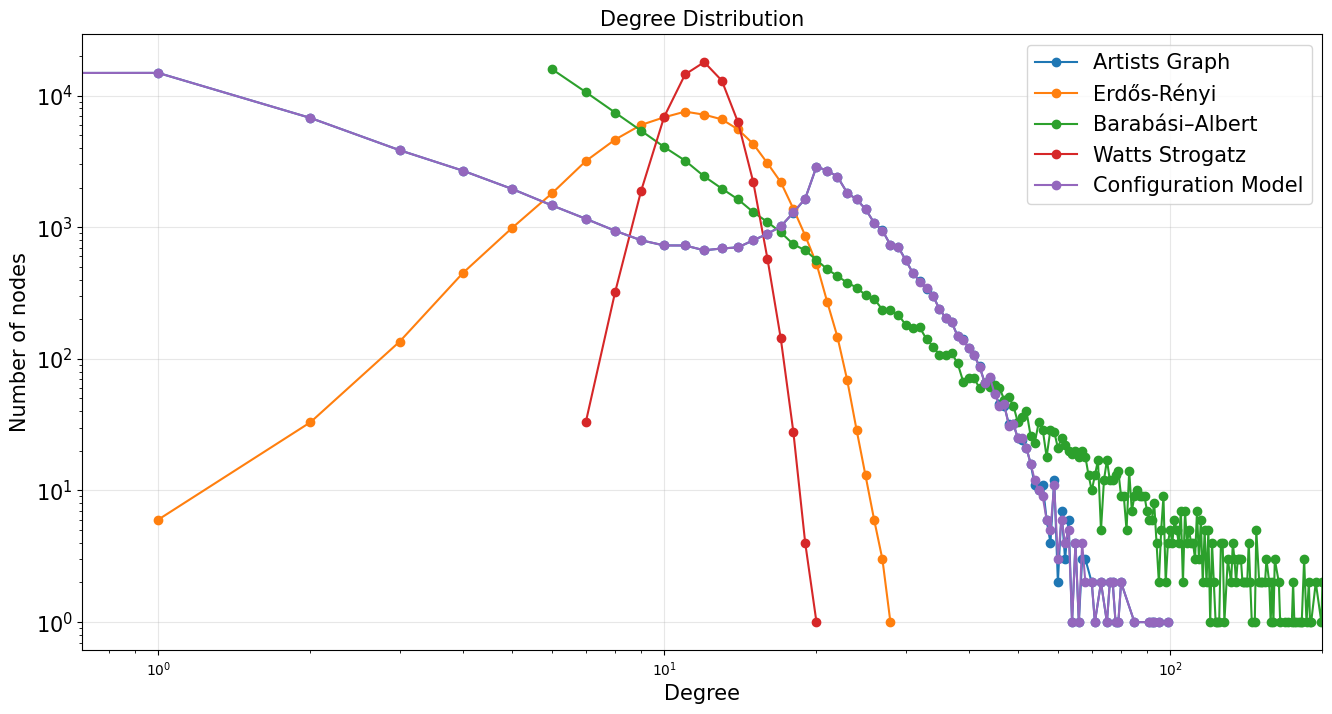
\includegraphics[width=7cm]{img/net_dist.png}
\caption{Degree distribution comparison}
\label{fig: Misogynous class distribution}
\end{figure}
% end figure

Analyzing the top nodes by degree in the artists network revealed a prevalence of classical performances, latin hip-hop and Indian film music as top genres - these being nodes that could be labeled as hubs for high degree thresholds. We can further analyze differences in terms of nodes highest/lowest degree with respect to synthetic graphs: relevant differences arise focusing on high degree nodes, as Table \ref{table:deg} suggests, with results consistent with the approaches used to build the synthetic networks. 

\subsection{Connected components analysis}
We also perform an analysis regarding connected components in both real world network and synthetic ones: a connected component can be identified as a sub-graph whose nodes can be reached from one another by following the network's links. For ER, WS and BA networks a single giant component equal to the whole original graph can be isolated. CM network presents a total of 168 components, the biggest one having 63399 nodes, with the remaining components having a much smaller cardinality of 1, 2 or 3 total nodes. The same pattern is identified in the AN networks, having 21 components, the biggest one including 63695 nodes and all the others at most 2 nodes. Following \cite[p. 59]{barabasi16}, the networks under analysis can be considered instances of connected regimes, where the average degree $\left \langle k \right \rangle$ is equal or very close to $ln(N)$\footnote{In our particular case, $ln(N)=11.062$.}, leading the vast majority or the totality of nodes to be encapsuled into a single giant component, still keeping the network relatively sparse.

\subsection{Clustering coefficient and assortativity}
The local clustering coefficient of a node can be considered as the proportion of the number of links between the nodes within its neighbourhood divided by the number of links that could possibly exist between them. When this value is close to one, it indicates how the node's neighbours are close to being a clique, or how complete the neighborhood of the node is. The average local clustering coefficient (Average CC), as the name suggests, provides insight regarding how complete the neighborhood of a node is, on average. All the synthetic models fail to correctly approximate the average clustering coefficients of the real world graph, which instead shows a much higher value, as depicted in Table \ref{table:density_comp}: this highlights how nodes in the artists network tend to have neighbours which form cliques more frequently then their synthetic counterparts.

% start figure
\begin{figure}[H]
\centering
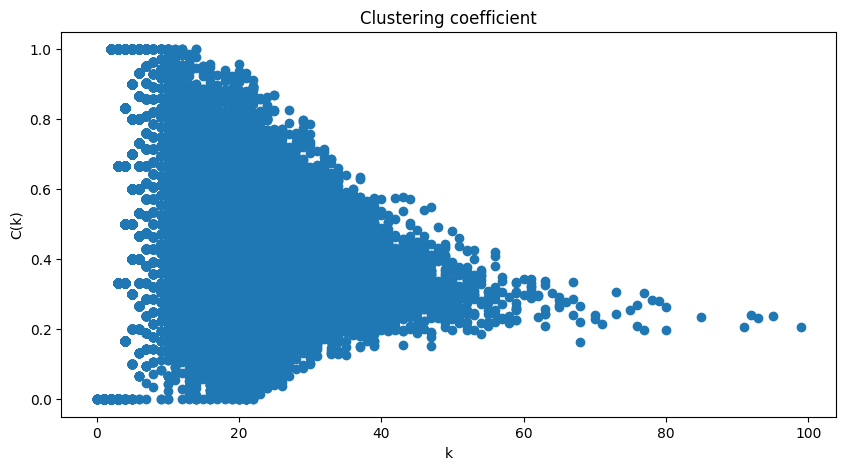
\includegraphics[width=7cm]{img/graph_clust_coeff.png}
\caption{Clustering coefficient distribution}
\label{fig: clust_distr}
\end{figure}
% end figure

\renewcommand{\arraystretch}{1.3}
\begin{table}[H]
\begin{center}
\scriptsize
\begin{tabular}{ |l|c|c|c|c| } 
 \hline
 \textbf{Model} & \textbf{Density} & \textbf{Average CC} & \textbf{\#Triangles} & \textbf{Assortativity}\\
 \hline
 AN & $18\cdot10^{-5}$ & 0.3962 & 3118005 &
 $0.1702$\\
 ER & $18\cdot10^{-5}$ & 0.0002 & 888 & $0.0016$\\
 BA &  $18\cdot10^{-5}$ & 0.0018 & 19068 & $-0.0144$\\
 WS & $19\cdot10^{-5}$ & 0.0002 & 1469055 & $-0.0135$\\
 CM & $18\cdot10^{-5}$ & 0.0005 & 4839 & $-3.1908$\\
 
 \hline
\end{tabular}
\end{center}
\caption{\label{table:density_comp} Density and clustering coefficient comparison between artists networks and synthetic networks}
\end{table}

As mentioned before, all the graphs show very low density values; the artists network is the one having the highest degree assortativity score, measuring the similarity of connections in the graph with respect to the node degree. We also leverage three nodes' features in order to provide further assortativity scores, measuring the similarity of the connections with respect to specific attributes. For this aim, we discretize the number of followers attribute into 250 bins using a quantile-strategy\footnote{All bins in each feature end up having the same number of points.}. The highest result is given by using the main genre of an artist as reference attribute (0.3358), while lower results were obtained for popularity (0.0191) and the discretized number of followers (0.01162).

% start figure
\begin{figure}[H]
\centering
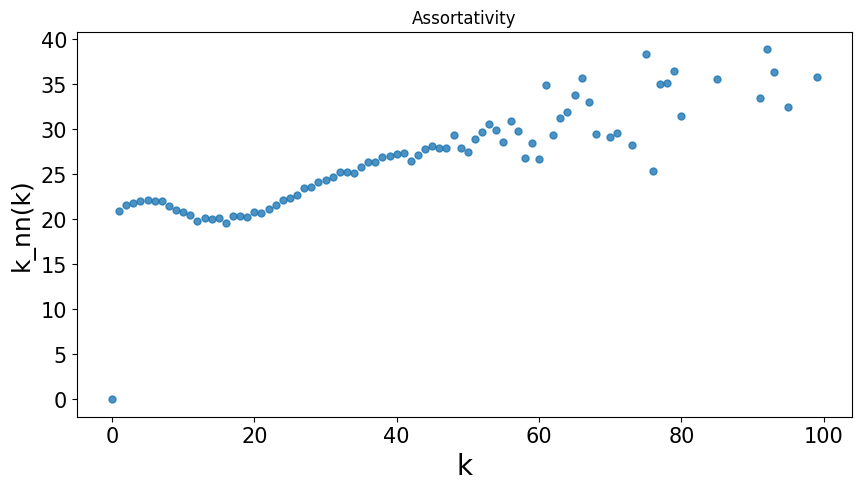
\includegraphics[width=7cm]{img/degree_assortativty.png}
\caption{Nodes correlation thorugh degree assortativity}
\label{fig: clust_distr}
\end{figure}
% end figure

\subsection{Path analysis}
Computing a large-size graph diameter and its average shortest path can be costly, as in our case. Therefore, we apply approximation methods in order to get an estimate of these real values computed on the respective biggest giant components. Following \cite{diam_app} and the 2-sweep algorithm implementation offered in Networkx library for undirected graphs, we pick the farthest node from a random node and return its eccentricity (i.e. length of a longest shortest path starting at that node) in order to obtain a lower bound on the diameter value. In order to compute an estimate for the average shortest path length, we leverage the following process: for each giant component, we randomly sample 200 pairs of nodes and compute their shortest path length, then we average the obtained values. We repeat the previous step 100 times, getting 100 average values coming from different samples of size 200. Their mean value represents our estimate for the average shortest path of the giant component under analysis. We report the obtained results\footnote{For the average shortest path length, results are in the form of mean of the samples$\pm$standard deviation.} in Table \ref{table:diam_short}.

\renewcommand{\arraystretch}{1.3}
\begin{table}[H]
\begin{center}
\scriptsize
\begin{tabular}{ |l|c|c|c|} 
 \hline
 \textbf{Model} & \textbf{2-sweep diameter} & \textbf{Appr. average shortest path} \\
 \hline
 AN & 23 & $8.7724\pm0.1308$ \\
 ER & $8$ & $4.7621\pm0.0407$\\
 BA &  6 & $3.9526\pm0.0367$ \\
 WS & 8 & $5.7999\pm0.0600$ \\
 CM & 12 & $4.5854\pm0.0550$ \\
 
 \hline
\end{tabular}
\end{center}
\caption{\label{table:diam_short} Approximated diameter and average shortest path length}
\end{table}

The artists network shows the highest average shortest path length, although presenting the highest standard deviation among the estimations made. This might be interpreted as the average number of jumps a user has to make to pass from one artist to a different one following the “Fans Also Like”-feature. In terms of diameter, the artists network shows again the highest value with respect to the other synthetic graphs, which present results in line with their topological inherent features.

\subsection{Centrality analysis}
We also try to identify the most relevant artists according to different centrality measures. We discuss results obtained with degree centrality (taking into account the number of neighbours of each node), pagerank centrality (computing a ranking of the nodes in the graph based on the structure of the incoming links), harmonic centrality (given a node $u$, its harmonic centrality is the sum of the reciprocal of the shortest path distances from all other nodes to $u$), eigenvector centrality (given a node with index $i$ in the adjacency matrix $A$ and the eigenvalue $\lambda$, its eigenvector centrality is the $i$-th element of the vector $x$ defined by $Ax=\lambda x$), closeness centrality (given a node $u$, the reciprocal of the average shortest path distance to $u$ over all $n-1$ reachable nodes).

% start figure
\begin{figure}[H]
\centering
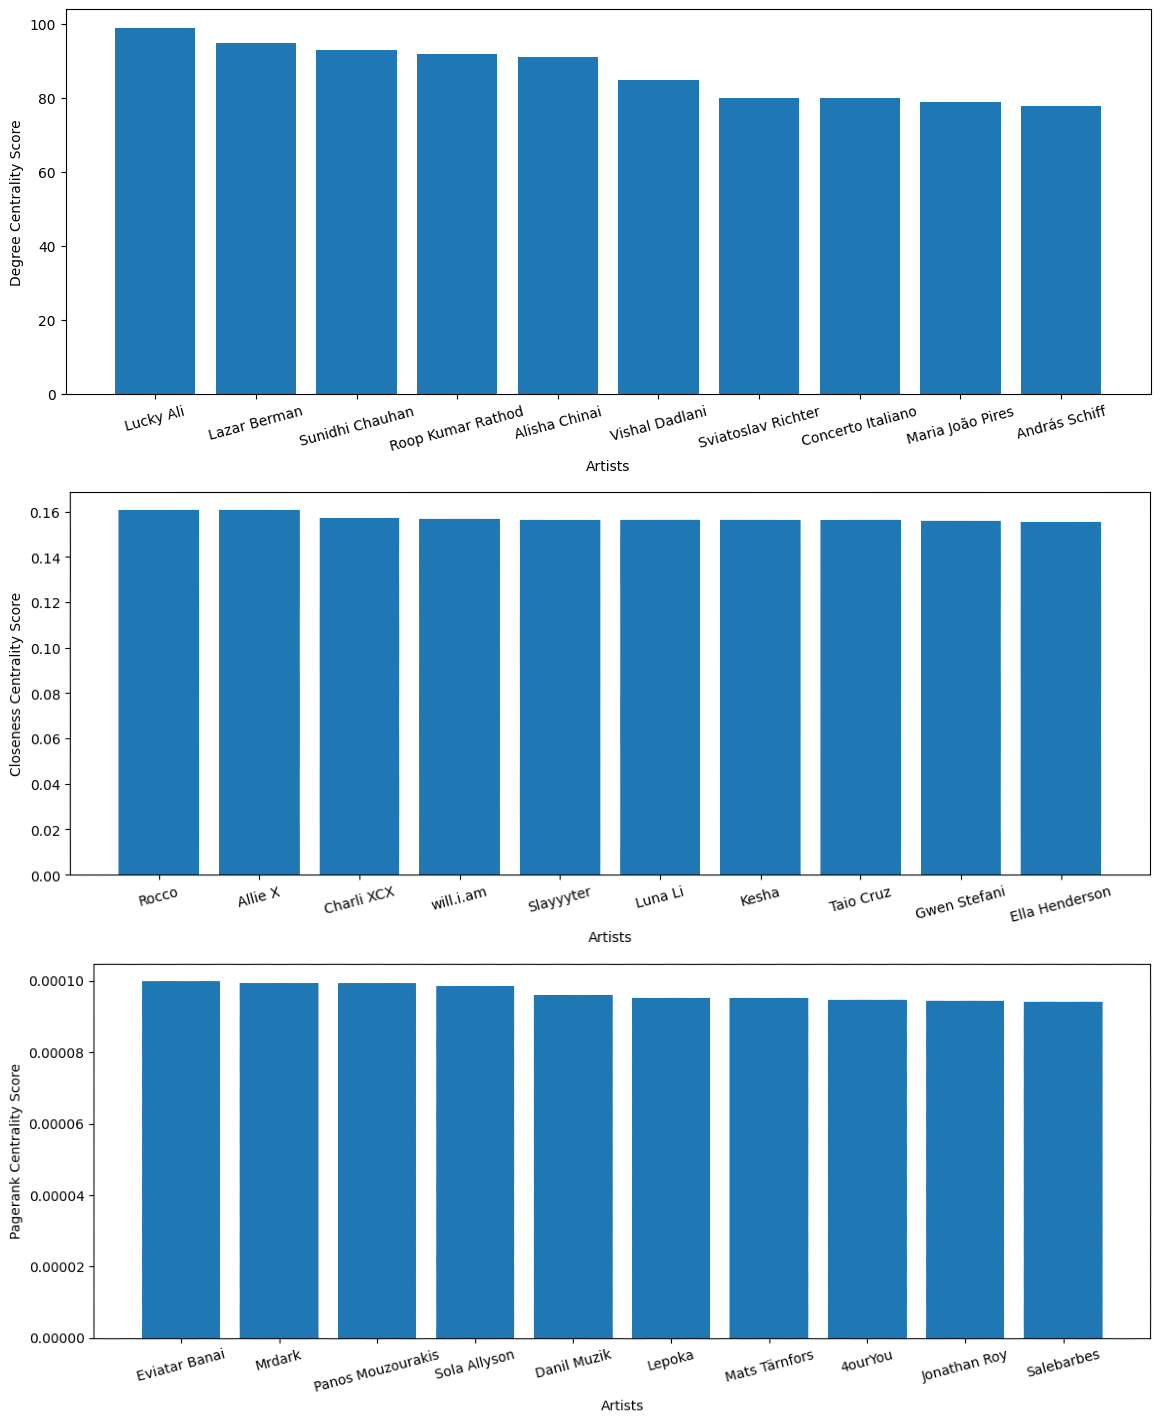
\includegraphics[width=7cm]{img/centr.png}
\caption{Top 10 nodes for degree, closeness and pagerank centrality}
\label{fig: clust_distr}
\end{figure}
% end figure

Focusing on the top results for each centrality measure, we mention how closeness and harmonic centrality measures match in terms of the top nodes identified, all of them belonging to the bedroom r\&b genre. Eigenvector and degree centrality measures match in terms of the top nodes, although in this case all of them belong to the Indian film music genre. Different results can be seen in terms of pagerank centrality, with most of the top nodes belonging to classic israeli pop genre.


\section{Task 1: Static Community Detection}
In this section we focus on a community detection task regarding the whole extracted artists network. For this purpose, we first take into account four different community detection algorithms, compare their performances in terms of internal and external evaluation metrics and then move to assess the nature of the clusters found by the best performing method among the ones under analysis.

\subsection{Internal evaluation}
We take into account the CDLIB\footnote{More information is offered in \cite{rossettih}.} implementation of Label Propagation, K-clique, Demon and Louvain community detection algorithms, performing for the last three a random search taking into account 3 instances of evaluation to find better parameters for the partitioning process, using Girvan-Newman modularity\footnote{More details a in \cite{girnew}.} for choosing the best parameters configuration. The best obtained parameters are shown in Table \ref{table:params_cdlib}\footnote{For K-clique we tested with $k$ from 2 to 10; for Demon, an $\epsilon$ from 0.1 to 0.9 with step=0.1 and a min. community size of 3,4,5; for Louvain, the randomize parameter with resolution from 0.1 to 0.9, with step=0.1.}. Table \ref{table:params_cdlib_2} completes the internal evaluation summarizing the obtained results.

\renewcommand{\arraystretch}{1.1}
\begin{table}[H]
\begin{center}
\scriptsize
\begin{tabular}{ |l|c|c|c| } 
 \hline
 \textbf{Algorithm} & \textbf{Parameters} & \textbf{\#Communities} & \textbf{Modularity}\\
 \hline
Label Propagation & - & 2027  & 0.7558 \\
 K-clique & $k=7$ & 1422  & $0.2520$\\
 Demon &  {min\_com\_size}=4, $\epsilon=0.2$ & 460 & $0.5688$\\
 Louvain &  res=0.6, rand=True & 89  & 0.9345\\
 
 \hline
\end{tabular}
\end{center}
\caption{\label{table:params_cdlib} Communities size, modularity and coverage comparison between tested algorithms}
\end{table}

\renewcommand{\arraystretch}{1.1}
\begin{table}[H]
\begin{center}
\scriptsize
\begin{tabular}{ |l|c|c|c| } 
 \hline
 \textbf{Algorithm} & \textbf{Cut ratio} & \textbf{Avg. internal degree} & \textbf{Conductance}\\
 \hline
Label Propagation & $4.09\cdot10^{-5}$ & 5.5681  & 0.3486 \\
 K-clique & $2.02\cdot10^{-4}$ & 10.5952  & $0.5303$\\
 Demon &  $6.68\cdot10^{-5}$ & 13.1771 & $0.2470$\\
 Louvain &  $4.27\cdot10^{-6}$ & 8.4918  & 0.0244\\
 
 \hline
\end{tabular}
\end{center}
\caption{\label{table:params_cdlib_2} Cut ratio, average internal degree and conductance comparison between tested algorithms}
\end{table}

Highest modularity scores (i.e  the fraction of edges within communities minus the expected fraction of
such edges) are obtained for Label Propagation and Louvain, which are also capable of covering the whole graph in terms of nodes without overlapping clusters. Furthermore, Louvain resulted the partitioning method with the lowest cut ratio (a measure indicating the possible number of links leaving the community) and lowest conductance (i.e the ratio between relationships that point outside a community $C$ and the total number of relationships of $C$): these properties, along with the one of  having a 100\% coverage of the graph's nodes and the relatively balanced average internal degree, make it the best partitioning method from the internal assessment process.

\subsection{External evaluation}
We compute the normalized mutual information between Label Propagation and Louvain results, having these two method a complete coverage over the graph and obtaining a score of 0.6941, indicating a partial overlapping between the two sets of communities identified. In order to analyze also community detection methods not covering the same set of nodes, we exploit the normalized F-1 score. Comparisons are shown in Table \ref{table:NF1}:

\renewcommand{\arraystretch}{1.3}
\begin{table}[H]
\begin{center}
\scriptsize
\begin{tabular}{ |l|c|c|c|c| } 
 \hline
 \textbf{Algorithm} & \textbf{Label Propagation} & \textbf{K-clique} & \textbf{Demon} & \textbf{Louvain}\\
 \hline
Label Propagation & - & 0.1018 & 0.0133 & 0.0030\\
 K-clique & 0.0779 & - & 0.0123 & 0.0014\\
 Demon &  0.0190 &0.0075& - & 0.0090\\
 Louvain & 0.0230 & 0.0088 & 0.0673 & -\\

 \hline
\end{tabular}
\end{center}
\caption{\label{table:NF1}Normalized F1 score of the algorithms partitions comparison}
\end{table}

All the scores are relatively low: the highest is given by Label Propagation compared with K-clique algorithm but we can't generally claim a relevant similarities between NF-1 results. 
We can exploit the additional semantic information regarding music genres attached to the graph's nodes for a deeper analysis of the Louvain communities results. For each node, we have a list of genre the artist is associated with along with its main genre. Computing the average purity\footnote{Here with purity of a community with respect to an attribute we mean the number of instances the most frequent label of that attribute has in that community, taken in percentage.} in terms of main genre gives us poor results ($24.56\%\pm11.56\%$, if we remove from the analysis the 20 Louvain communities having a size smaller then 3), but this should not be immediately linked with poor clustering results in general: there is a total of 4728 different genres in the graph, rendering the attempt to make sense of the obtained clusters in terms of these fine-grained labels unreliable. In fact, switching to a more coarse-grained approach gives us more reasonable results: for each community, we evaluate for each genre how many times it occurs in one of the genre sets associated with each artist in the community, taking the value in percentage with respect to the community size. As expected, this approach leads to more reasonable results: even if most of the communities obtained tend to show a majority of not available genre as their most frequent genre, ,many results make sense regarding intuitive semantic similarity between the genres that tend to recurr the most in the community. Some interesting examples are shown in Table \ref{table:genres}. Even if just approximately, we can claim that Louvain is also able to capture homogenous clusters in terms of coarse-grained information regarding genre.

\renewcommand{\arraystretch}{1.3}
\begin{table*}[]
\begin{center}
\scriptsize
\begin{tabular}{ |l|c|c|} 
 \hline
 \textbf{Community label} & \textbf{Size} & \textbf{Top 5 genres in lists} \\
 \hline
59 & 143  & ('death metal', 59.44\%), ('brutal death metal', 51.75\%),
 ('deathgrind', 41.96\%),
 ('technical death metal', 34.27\%),
 ('grindcore', 30.77\%)\\
 38 & 665  & ('italian adult pop', 21.80\%),
   ('italian pop', 18.16\%),
   ('classic italian pop', 17.44\%),
   ('italian hip hop', 15.49\%),
   ('genre not available', 11.43\%)\\
 31 & 827  & ('k-pop', 27.90\%),
   ('korean pop', 20.69\%),
   ('k-rap', 15.96\%),
   ('genre not available', 11.35\%),
   ('k-indie', 10.40\%)\\
54 & 261  & ('bebop', 31.42\%),
   ('jazz', 26.82\%),
   ('hard bop', 22.61\%),
   ('background jazz', 22.22\%),
   ('jazz saxophone', 17.62\%)\\
   
3 & 2171  & ('genre not available', 18.19\%),
   ('j-pop', 8.34\%),
   ('j-rock', 8.20\%),
   ('anime', 6.96\%),
   ('j-rap', 5.02\%)\\

0 & 3553  & ('genre not available', 10.86\%),
   ('pop', 4.93\%),
   ('r\&b', 4.84\%),
   ('alternative ', 4.59\%),
   ('hip hop', 3.86\%)\\

29 & 900  & ('mpb', 18.11\%),
   ('samba', 15.88\%),
   ('bossa nova', 14.88\%),
   ('pagode ', 14.44\%),
   ('velha guarda', 11.44\%)\\

10 & 1827  & ('genre not available', 13.19\%),
   ('chanson', 8.81\%),
   ('french rock', 5.74\%),
   ('nouvelle chanson francais', 4.81\%),
   ('trip hop', 4.59\%)\\

   
 \hline
\end{tabular}
\end{center}
\caption{\label{table:genres}Examples of most frequent genres in artist genre lists}
\end{table*}

% start figure
\begin{figure}[H]
\centering
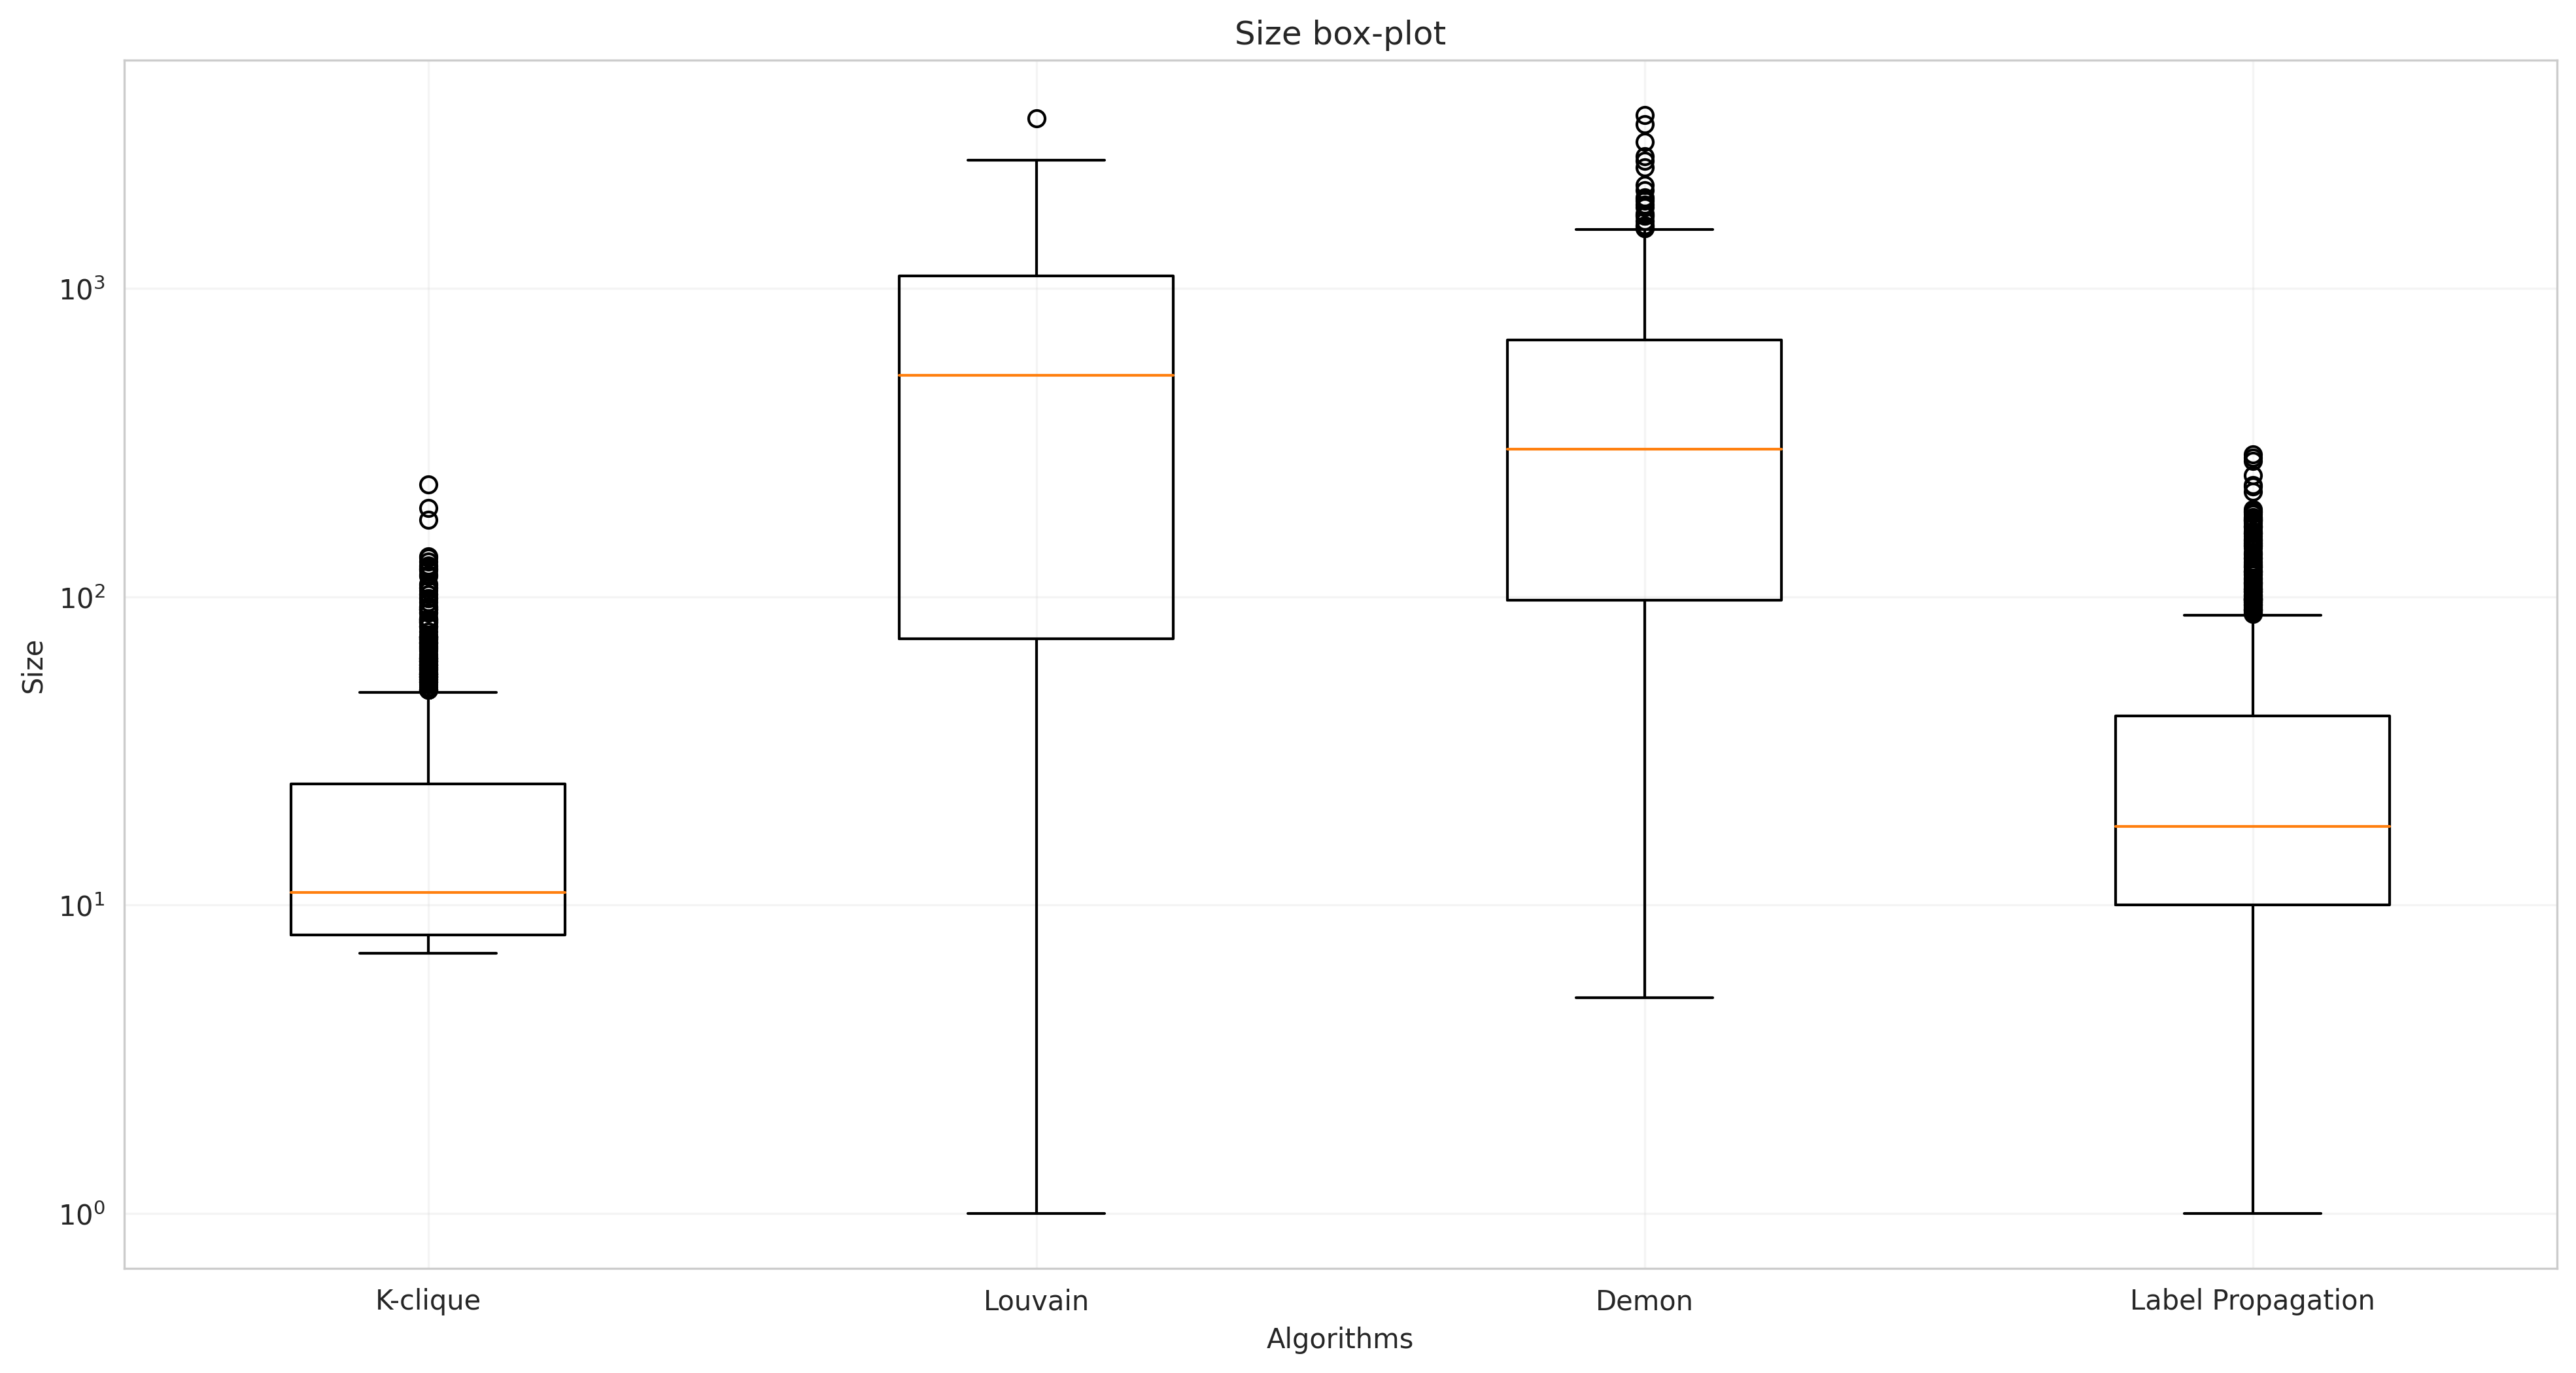
\includegraphics[width=7cm]{img/boxplot_size_comm.png}
\caption{Algorithms comparison in terms of size}
\label{fig: boxplot_community}
\end{figure}
% end figure

% start figure
\begin{figure}[H]
\centering
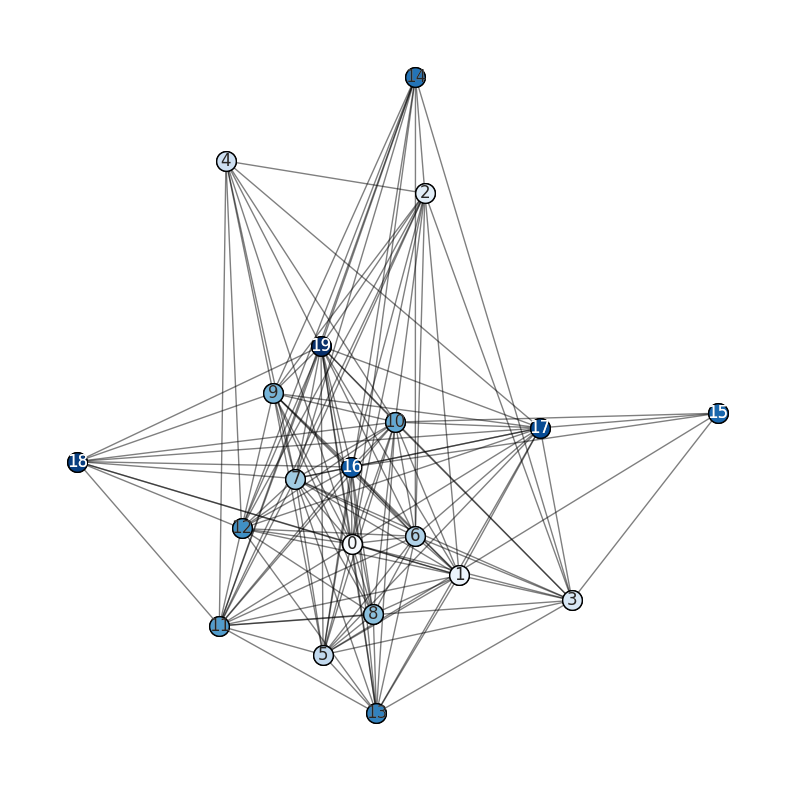
\includegraphics[width=7cm]{img/louvain_graph.png}
\caption{Visualization of top 20 Louvain communities relationships}
\label{fig: boxplot_community}
\end{figure}
% end figure

% start figure
\begin{figure}[H]
\centering
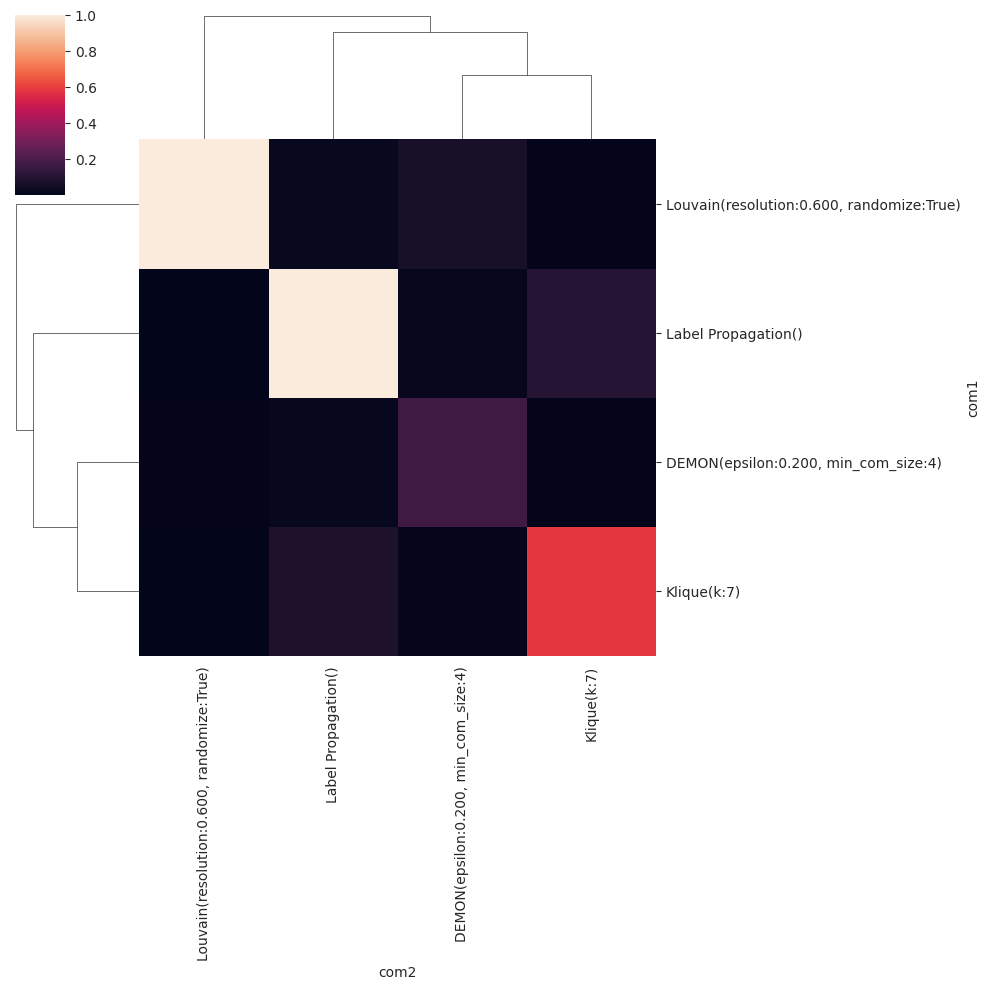
\includegraphics[width=5cm]{img/normalized_mi.png}
\caption{NF-1 comparison matrix between algorithms}
\label{fig: NMINFO}
\end{figure}
% end figure



\section{Task 2: Link prediction}
The goal of this section is understanding to what extent and precision it is possible to predict potential connections between unlinked nodes inside the artists network. We tackle the problem from two distinct perspective: using unsupervised tools (relying on inherent topological structure of the network to solve the task without taking into account any ground-truth information to learn from) and supervised ones (exploiting "traditional" supervised machine learning methods, learning a model from a proper labeled data representation in order to test its performance on not already seen observations).

\subsection{Unsupervised link prediction}
We chose to test three unsupervised methods focusing on nodes' topology, these being Common Neighbors, Jaccard similarity, and Adamic Adar, and a link-based similarity approach, namely SimRank\footnote{A deeper explanation regarding the measures can be found in \cite{nowellklein}.}. In Common Neighbors, the score for link prediction is computed by finding the number of common neighbors between two distinct nodes as follows, assuming that nodes sharing many common neighbors should also be linked themselves:

\begin{equation}
    CN(u,v) = |{N_u\cap N_v}|
\end{equation}

Jaccard similarity assumes that nodes sharing many neighbors over their merged common neighborhoods should be similar, hence connected:

\begin{equation}
    Jaccard(u,v) = \frac{|N_u\cap N_v|}{{|N_u\cup  N_v|}}
\end{equation}

Adamic Adar takes into account nodes' degrees, giving higher impact to lower degree nodes and lower impact for hubs. More specifically, higher degree nodes could appear more frequently in the same neighborhood then nodes with less degree, hence the former should contribute less to the score then the latter:

\begin{equation}
    AA(u,v) = \sum _{k\in{N_u}\cap {N_v}}\frac{1}{log(|N_k|)}
\end{equation}

SimRanks follows a different rationale, assigning a likelihood of observing a link between two nodes analysing the similarity of their respective neighbourhoods:

\begin{equation}
    SR(u,v) = C \frac{\sum_{k\in{N_u}}\sum_{k'\in{N_v}}SR(k,k')}{|N_u|\cdot |N_v|}
\end{equation}

where $C$ is a decay factor in the range $[0,1]$.

Due to the high computational cost of these methods\footnote{The problem is mainly related to the necessity of computing every possible edge given a set of nodes: in fact, most methods we will deal with imply a not-optimal $O(|V|^2)$ cost, where $V$ is the number of nodes in the network.}, we employ a sub-graph of the original network, including only nodes having a degree higher or equal to 40 and excluding from the obtained sub-graph nodes belonging to components having cardinalities lower then 5. This allows us to reduce the analysis over a graph comprised of 666 nodes and 2582 edges: 225 were used during testing phase and the remaining one for the training of the unsupervised methods. Figure \ref{fig:roc_sup_jac} reveals the low performances concerning topology oriented methods on the analyzed sub-graph: Jaccard Similarity is slightly above the other two considered methods in terms of ROC-AUC, but still unsatisfactory, even if it shows the best trade-off between Precision and Recall scores focusing of PR-AUC. 
A relevant change in performances can be observed studying SimRank results, as shown in Figure \ref{fig:roc_sup_simrank}: we employed three different decay factor values, each of them showing roughly the same performances in terms of ROC-AUC and shared top predictions. Using $C=0.3$ seems to lead to slightly better results in terms of Precision-Recall trade-off, hence we will focus on this method for further comparisons. We observe how each SimRank evaluation lead to optimal results once compared with a random link prediction classifier. Table \ref{table:uns_inters} completes the analysis showing the top 250 shared predictions among the unsupervised methods, highlighting the similarities between Adamic Adar results and Common Neighbors and Jaccard with SimRank with $C=0.3$.

\renewcommand{\arraystretch}{1.3}
\begin{table}[H]
\begin{center}
\scriptsize
\begin{tabular}{ |l|c|c|c|c| } 
 \hline
 \textbf{Method} & \textbf{Common N.} & \textbf{AdamicAdar} & \textbf{Jaccard } & \textbf{SimRank}\\
 \hline
 Common N. & 250 & 205 & 59 & 0\\
 AdamicAdar  & 205 & 250 & 93 & 4\\
 Jaccard  &  59 & 93 & 250 & 127 \\
 SimRank & 0 & 4 & 127 & 250 \\

 \hline
\end{tabular}
\end{center}
\caption{\label{table:uns_inters}Number of shared predictions among the top 250 scores across unsupervised methods}
\end{table}

\begin{figure}[H]
\centering
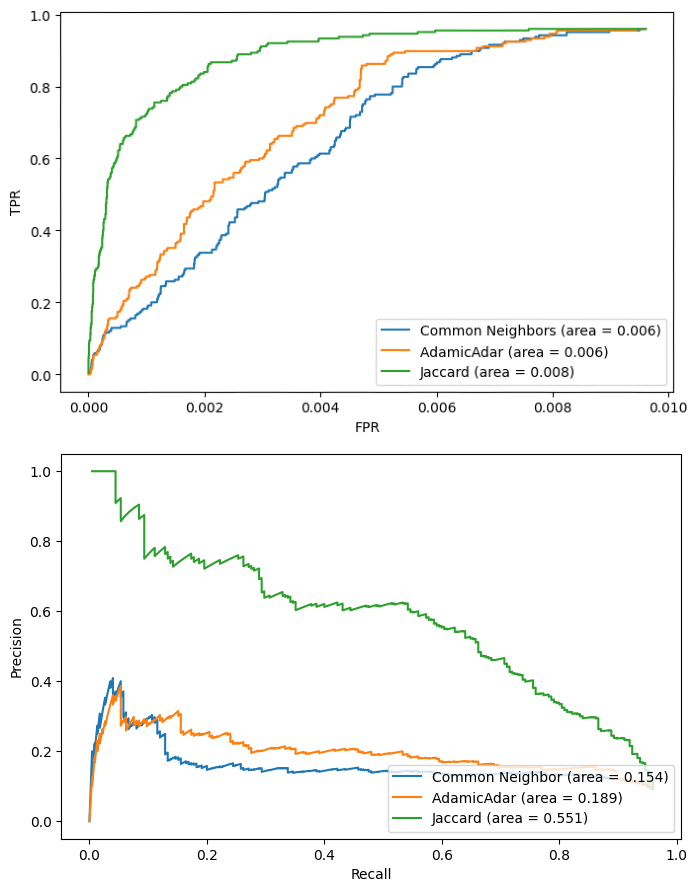
\includegraphics[width=7cm]{img/roc_jac3.png}
\caption{ROC curves and Precision-Recall curves for Common Neighbors, Jaccard and Adamic Adar methods}
\label{fig:roc_sup_jac}
\end{figure}

\begin{figure}[H]
\centering
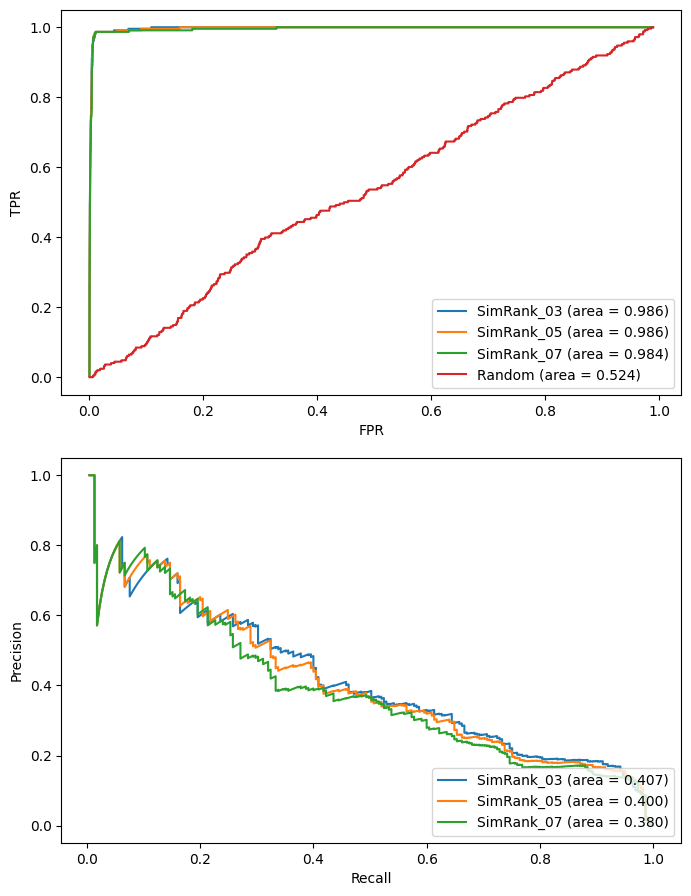
\includegraphics[width=7cm]{img/roc_sim3.png}
\caption{ROC curves and Precision-Recall curves for SimRank method}
\label{fig:roc_sup_simrank}
\end{figure}



\subsection{Supervised link prediction}
We also explore solutions regarding supervised approaches, implementing traditional machine learning models for link prediction. We employ StellarGraph library\footnote{More information available at https://github.com/stellargraph/stellargraph, \cite{StellarGraph}.} in order to sample positive and negative links from the initial graph (where a positive label identifies the actual presence of that link, a negative label its absence), splitting the graph into a training set (50451 node pairs) and test set (74742 node pairs), setting 10\% as percentage of links to be sampled from the starting graph. We encode the graphs obtained into Node2Vec embeddings\footnote{More information available at https://github.com/aditya-grover/node2vec, \cite{node2vec-kdd2016}.}, using second-order random walks to generate sentences (i.e. list of node ids) from the training graph and learning an embedding vector for each word (i.e. node id). We build feature representations for links applying binary operators on the pair of embeddings associated to nodes forming that link, considering Hadamard, Average, L1 and L2 operators as described in \cite{jorgschl}. We take into account three ML models\footnote{We consider the implementation offered in Scikit-learn library. More detailed information is offered in \cite{Pped}.}: K-Nearest Neighbors (K-NN)\footnote{Testing (3,5,7,9,11) as possible $k$s, giving uniform weights to the points or weighting them by their distance.}, Decision Tree (DT)\footnote{Testing Gini and Entropy as splitting criteria, (2,4,6,8,10) as min\_samples\_split (minimum number of samples required to split a node) and (1,2,3,5,8,10) as min\_samples\_leaf (minimum number of samples required to be a leaf node).}  and Logistic Regression (LR)\footnote{Testing L2,L1 and no penalty, (1.0,0.0,0.001) as $C$s and newton-cg, liblinear and lbfgs solvers. In case of configurations with incompatible hyperparameter values, we simply skip them in the grid search process.}. For each solver, a gridsearch using a stratified $k$-fold cross validation approach with $k=5$ in order to identify the best parameters for each particular class of models has been performed, considering different feature spaces obtained from different binary operators. As scoring criterion considered for the extraction of the best model, accuracy has been chosen. Models reported in Table 1 are the ones with the highest mean score over the validation folds\footnote{Results are in the form of accuracy $\pm$ standard deviation, for validation scores.} according to their respective gridsearch, for each feature space.

\begin{table}[H]
  \centering
  \renewcommand{\arraystretch}{1.2}
  \resizebox{\columnwidth}{!}{
  \begin{tabular}{|p{2cm}|c|c|c|c|c|c|c|c|c|}
    \hline
    \textbf{{Feature Space}} & \multicolumn{2}{c|}{\textbf{Logistic Regression}} & \multicolumn{2}{c|}{\textbf{Decision Tree}}
    & \multicolumn{2}{c|}{\textbf{K-Nearest Neighbors}}
    
    
    \\
    % \hline
    % \textbf{Inactive Modes} & \textbf{Description}\\
    \cline{2-7}
    & \textbf{Mean VL} & \textbf{TS} & \textbf{Mean VL} & \textbf{TS}
    & \textbf{Mean VL} & \textbf{TS} 
    \\
    %\hhline{~--}
    \hline
    {Hadamard} & $96.90\%\pm0.13\%$ & $96.91\%$ & $88.58\%\pm0.20\%$  & $88.67\%$ &  $96.75\%\pm0.11\%$  & $96.70\%$  \\ \hline
    {Average} & $65.88\%\pm0.40\%$ & $66.60\%$ &$83.49\%\pm0.25\%$ & $84.52\%$ & $95.47\%\pm0.24\%$ & $95.63\%$  \\ \hline
    {L1} & $94.42\%\pm0.15\%$ & $94.49\%$ & $86.60\%\pm0.33\%$ & $87.01\%$ & $86.69\%\pm0.18\%$ & $87.65\%$ \\ \hline
    {L2} & $94.32\%\pm0.17\%$ & $94.41\%$ & $86.55\%\pm0.24\%$ & $87.05\%$ & $85.22\%\pm0.35\%$ & $86.30\%$ \\  
    \hline
  \end{tabular}
} 
\caption{Supervised link prediction task: validation and assessment results for each model and binary operators}
\label{table:stand_bin}
\end{table}

Hadamard operator provided the best results for every method considered: LR with lbfgs solver, $C=0.001$ and L2 penalty proved to be the best method in testing phase in terms of accuracy, followed by K-NN using $k=3$ and weighting points by the inverse of their distance and at last by DT with Gini splitting criterion 2 as min\_samples\_leaf and 8 as min\_samples\_split. ROC-AUC values for each testing result is provided in Figure \ref{fig:roc_sup}, emphasizing the goodness of each result. Even if LR resulted the best model in terms of Accuracy, a better trade off in terms of false positive and true positive rates is given by K-NN, which shows a slightly better AUC-score.

\begin{figure}[H]
\centering
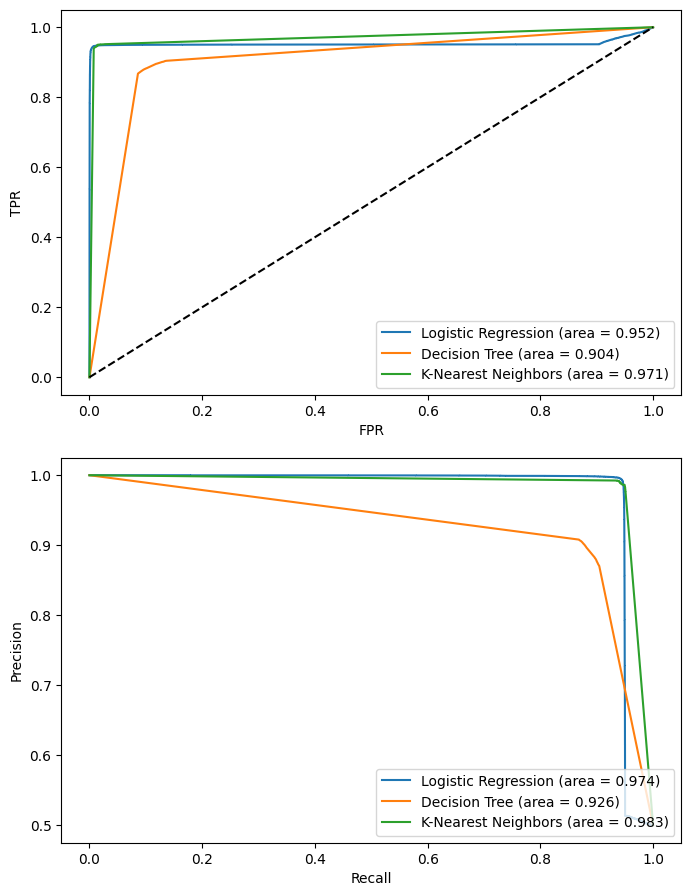
\includegraphics[width=7cm]{img/roc_superv_3_1.png}
\caption{ROC curves and Precision-Recall curves for supervised methods}
\label{fig:roc_sup}
\end{figure}

The results are completed by Table \ref{table:prec_rec}, reporting Precision, Recall and F1 scores regarding the presence of links for the test set in the Hadamard feature space, emphasizing the difference between the three methods.

\renewcommand{\arraystretch}{1.3}
\begin{table}[H]
\begin{center}
\scriptsize
\begin{tabular}{ |l|c|c|c| } 
 \hline
 \textbf{Methods} & \textbf{Precision} & \textbf{Recall} & \textbf{F1} \\
 \hline
Logistic Regression & 99.16\% & 94.61\% & 96.83\% \\
Decision Tree & 89.03\% & 88.20\% & 88.61\%\\
K-Nearest Neighbors & 98.62\% & 94.73\% & 96.64\% \\

 \hline
\end{tabular}
\end{center}
\caption{\label{table:prec_rec}Precision, Recall and F1 score of each solver on the Hadamard feature space for the test set}
\end{table}

\section{Task 4: open question}

As an open research question, we tackle the issue of understanding if album covers released by each artist are coherently related to music genres the artist is associated with, following the identification made through Louvain community discovery algorithm. After having extracted for each artist the first accessible album cover image through Spotify API\footnote{A total of 63415 over 63717 images were extracted: some albums lead to Spotify extraction problems and were simply discarded in the process.}, we proceed with solving an image classification task, an image sentiment classification task and a topic modeling task for images. We then complete the section with a simple analysis of the performance of two convolutional neural network (CNN) architectures trying to solve the prediction task of associating to each album the genre of the artist who released that album.

\subsection{Image and visual sentiment classification task}
We use a pre-trained version of Vision Transformer model as illustrated in \cite{dosovitskiy2021image}\footnote{Implementation available at \nolinkurl{https://huggingface.co/docs/transformers/model_doc/vit}} in order to assign to each album a label that should represent its visual content: the transformer is directly trained on image patches without the aid of convolutional layers and it is a sufficiently viable tools for our purpose. For the visual sentiment task, we use a modified pre-trained version of AlexNet for visual sentiment analysis as developed in \cite{Vadicamo_2017_ICCV}\footnote{Implementation available at https://github.com/fabiocarrara/visual-sentiment-analysis}: the authors trained a visual sentiment classifier starting from a set of user-generated tweets containing both texts and images, leveraging on the sentiment polarity of the textual contents to train such model. We report here some quantitative results comparing the communities in terms of purity of genres, sentiment and image kind: the Spearman correlation coefficient and respective p-value checking the purity correlation between communities in terms of image content and genre, sentiment and genre and image content and sentiment are respectively -0.075 and 0.537, 0.077 and 0.525, 0.147 and 0.225. Hence no evident correlation is present in terms of purities, as shown visually with the scatter plots in Figure \ref{fig: scatters}.

% start figure
\begin{figure}[H]
\centering
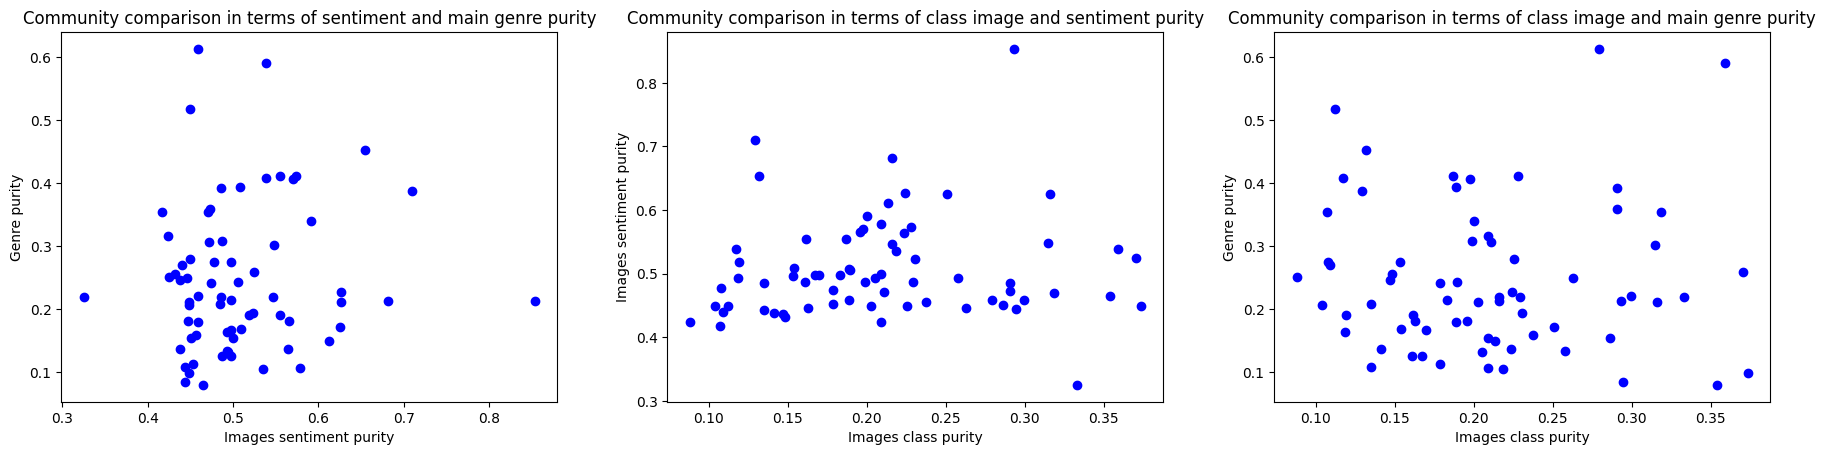
\includegraphics[width=8.5cm]{img/scatters.png}
\caption{Scatter plots comparing purity values in terms of genre, sentiment and image content}
\label{fig: scatters}
\end{figure}
% end figure

To complete the analysis, we mention how the top 10 communities in terms of sentiment purity (having more then 57\% of overall internal purity, with a max purity of 85\%) comprise a majority of positive images each and can be identified in order as sertanejo, lagu jawa, mexican music, albanian pop, indian pop, funk, tamil pop, cumbia villera, israeli pop and reggaeton. We also directly check the top 5 communties in terms of image content purity (having more then 33\% of internal purity, with a max purity of 37\%), these respectively having as most frequent contents book jacket,  dust cover, dust jacket, dust wrapper or comic book. Lower levels of purity for the image classification task are understandable, given the higher number of labels and image variety inside the same community.

\subsection{Topic modeling on images}
For a complete understanding of the albums characteristics with respect to the found communities, we use Concept Python library\footnote{Implementation available at \nolinkurl{https://github.com/MaartenGr/Concept}} in order to perform topic modeling on images, finding in an unsupervised way clusters of images sharing the same semantic visual content. Using Concept, we leverage CLIP (Contrastive Language-Image Pre-training)\footnote{More details in \cite{radford2021learning}.} approach along with BERTopic\footnote{Details in \cite{grootendorst2022bertopic}.} methods using transformers to create dense clusters of interpretable topics.

We perform a community-wise analysis, looking for prototypical combinations of images in the album cover of particularly homogeneous community in terms of music genres. The aim is understanding if intuitive semantic properties associated to music genres are coherently reflected and captured by the concept modeling procedure employed: for this reason we first analyze communities having both a sufficiently high cardinality to carry on the task and still keeping a somehow pure genre distribution at the same time\footnote{The concept library did not provide meaningful results for very small communities, these being also the purest for the trivial reason of being rather small.}. Some relevant examples are shown in Figure \ref{fig: cover_1}: each clusters of merged images captures the two or many main concepts identified by the approach\footnote{Information regarding community sizes and genres distributions used for the concept modeling examples are reported in Table \ref{table:genres}}. The first row focuses on the 54th community, showing how the album covers tend to represent either musicians playing classical jazz instruments or more abstract figures/natural environments. The second and third row focuses on the 31st community with the main concepts either capturing the frequency of albums displaying korean boy bands or idols and the other ones having more artistic representation or close-up photos of the artists. The fourth row displays the main concepts for brazilian popular music, focusing either on close-up images of artists or covers more abstract art representation. The last one is focused on the 14th community, showing an opposition between a more urban/street scenario concept and another one focusing on artists close-ups. On the other hand, in Figure \ref{fig: cover_2} we focus on communities with less pure genre distribution but far more samples. The first eight concepts capture the pop/hip-hop community, the biggest community: reasonably, most concepts are characterized by close-up or full length photos of both male and female artists, with a sub-set of cluters focused on more artistic visual representations. The second cluster of 7 images covers the  5th community, mainly including concepts regarding the j-pop and anime music: as one could intuitively expect, we have a concept  characterized by Japanese ideograms and a different one characterized by cartoonish female figures along with other topics either focused on idol boy bands, female artists close-ups and artistic visuals. The last 6 concepts characterize the french chanson albums, focusing on male or female performers close-ups. In summary, a clear general tendency can be identified: most albums for each genre identified through Louvain community tend to include at least two separate topics that describe them: one more focused on the artist depiction or the group associated to that album and a distinct one more characterized by abstract or visually captivating representations.

% start figure
\begin{figure}[H]
\centering
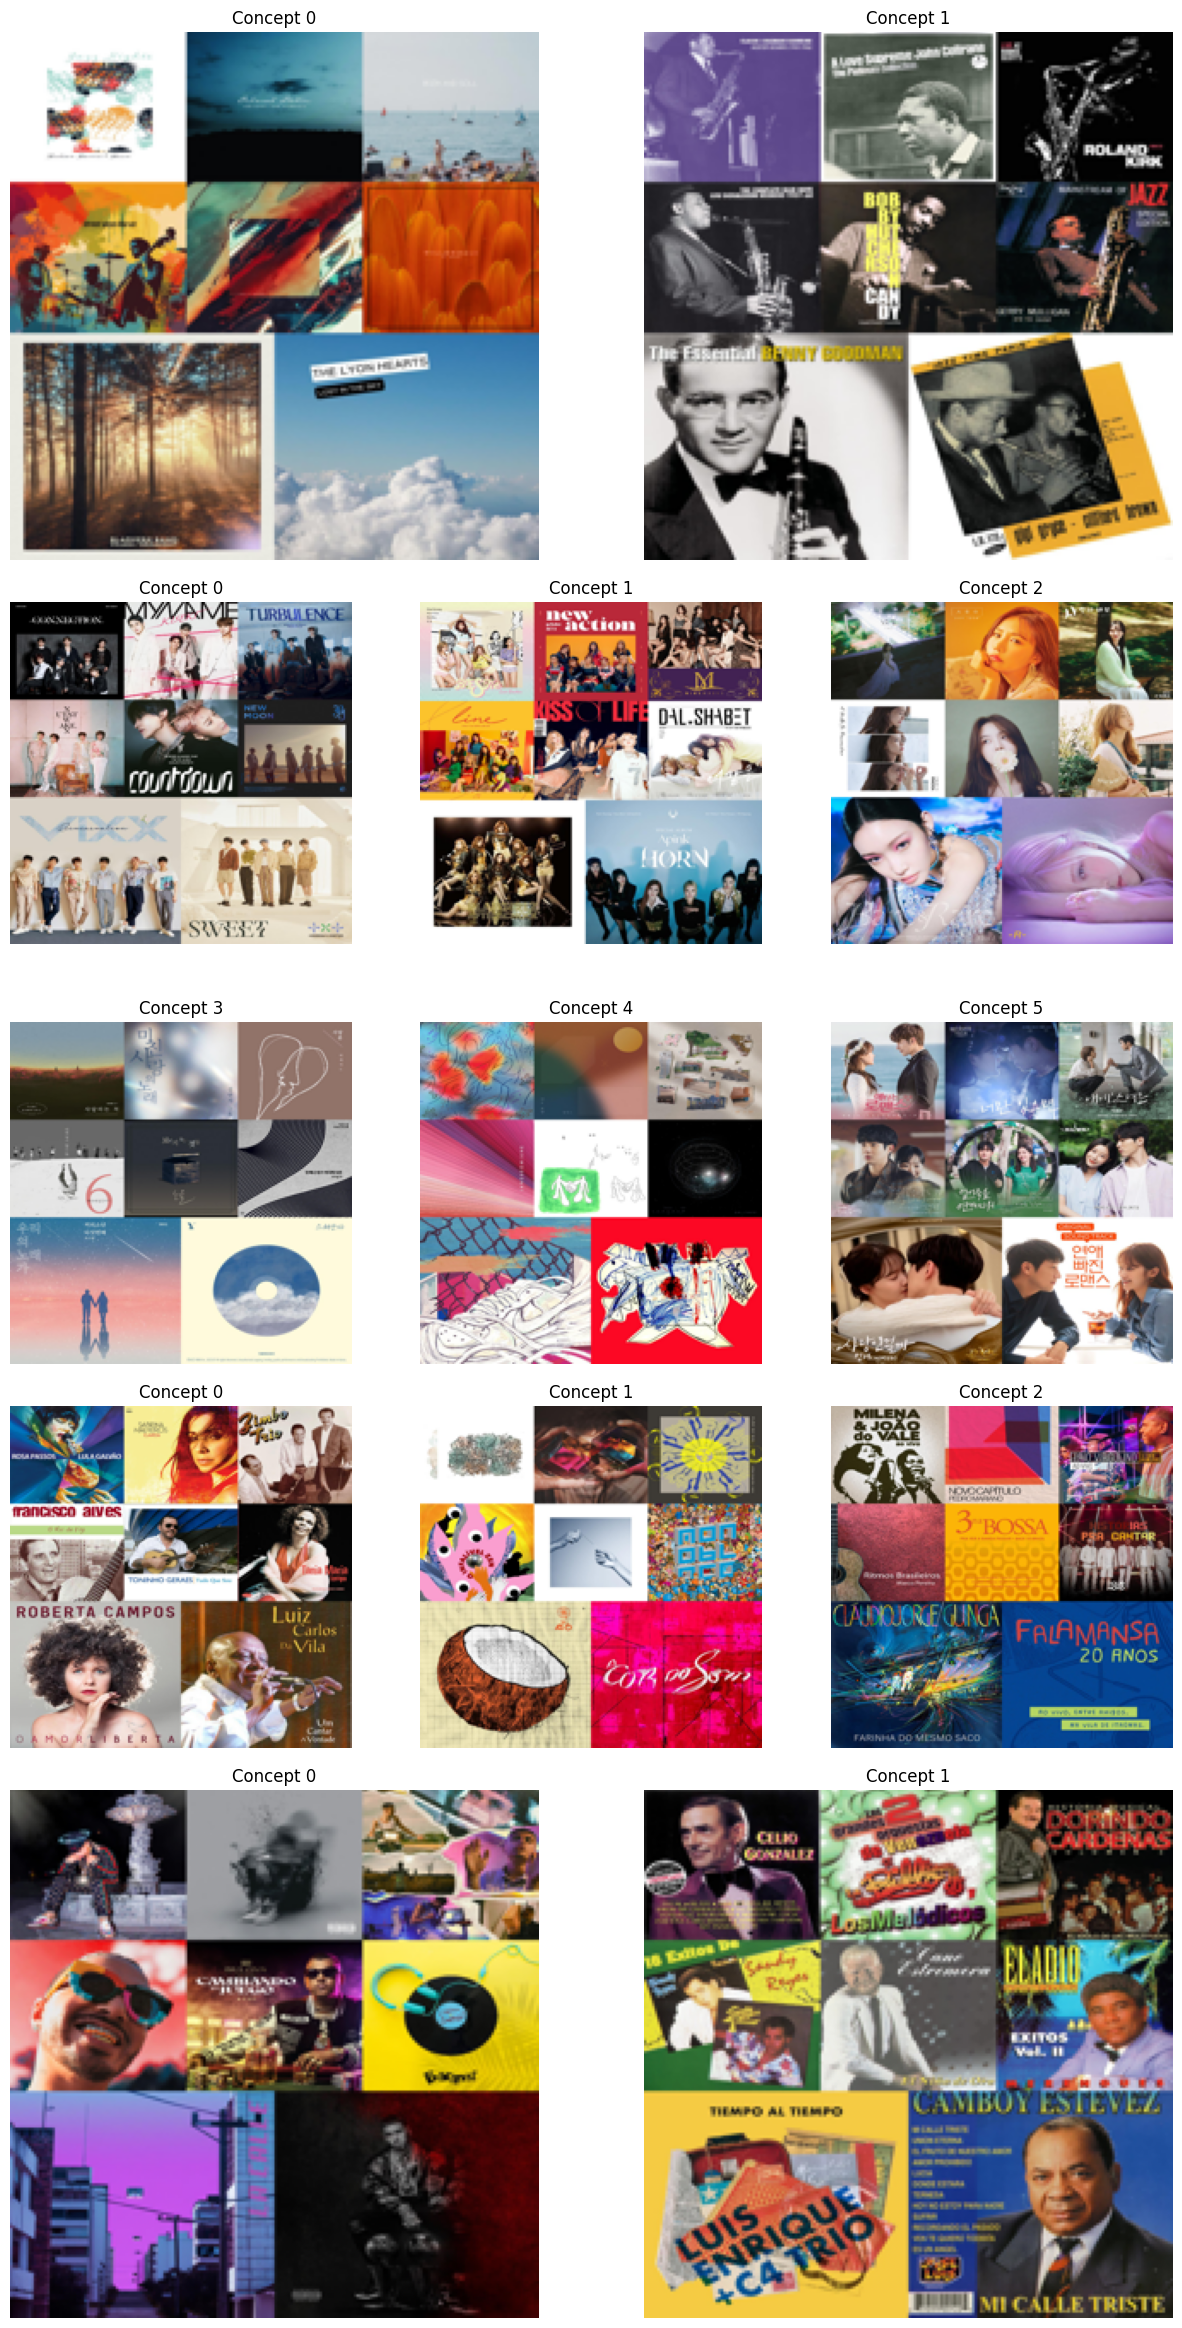
\includegraphics[width=6.5cm]{img/pic_1.png}
\caption{Concept modeling obtained from four relatively pure communities: the main genres are respectively bebop, k-pop, brazilian popular music, urbano latino}
\label{fig: cover_1}
\end{figure}
% end figure

% start figure
\begin{figure}[H]
\centering
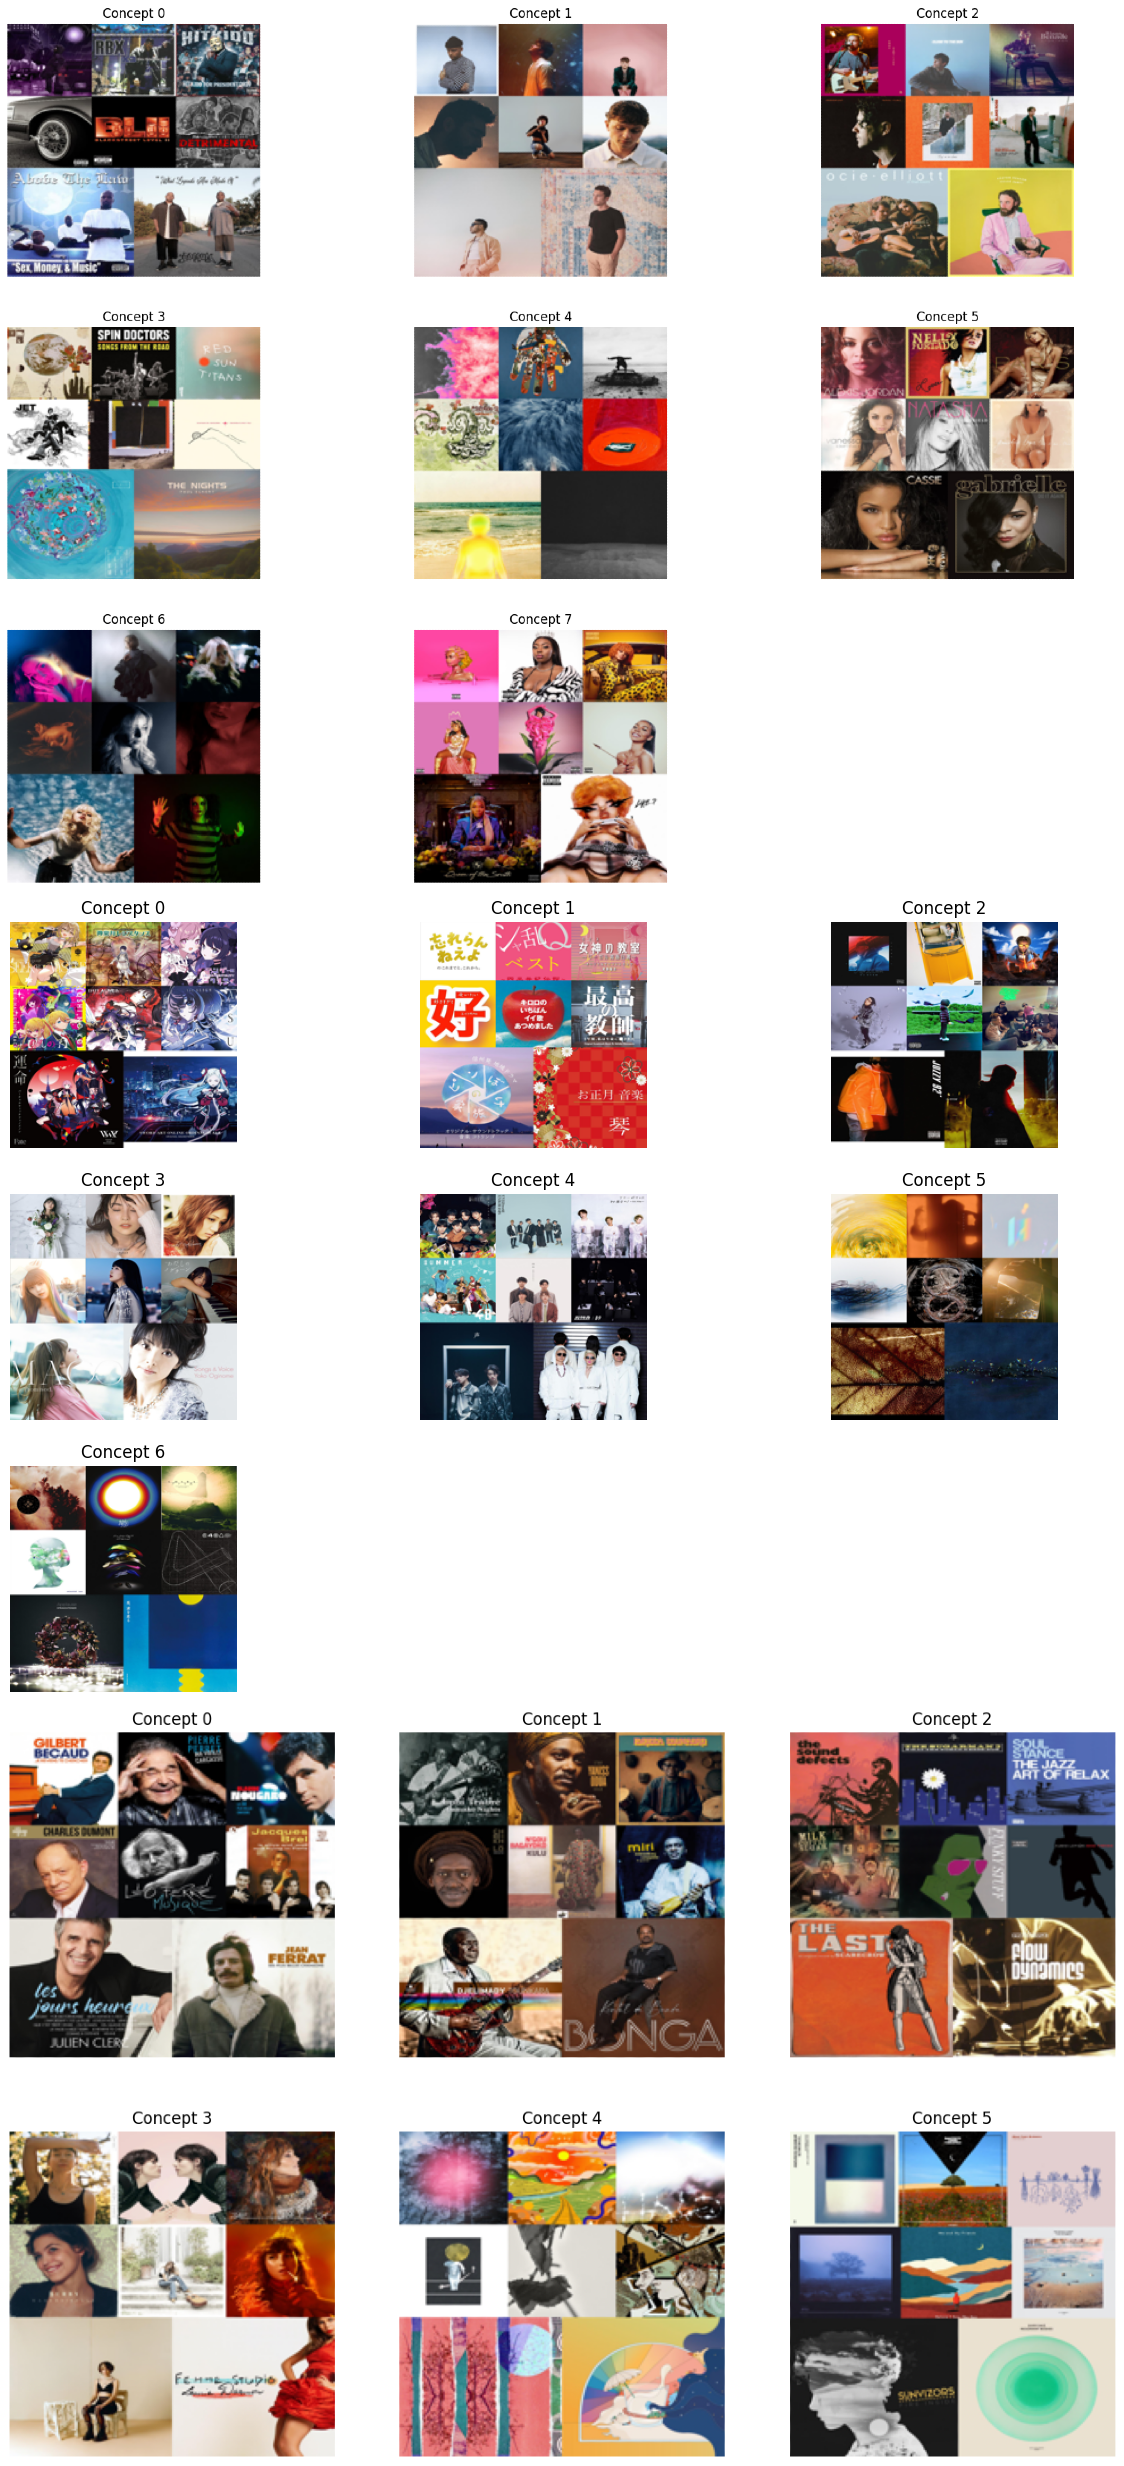
\includegraphics[width=6.5cm]{img/pic_2.png}
\caption{Concept modeling obtained from three communities of relevant size: the main genres are respectively pop/hip-hop, j-pop/anime music and french chanson}
\label{fig: cover_2}
\end{figure}
% end figure

\subsection{Learning a CNN to predict music genres from album covers}
The last task of our open question aims at investigating if a simple model can be trained on album covers in order to predict the genre associated with the artist's specific album. For this task, we first define a simpler multi-class problem: for each community, we identify the album associated to each artists belonging to such community and assign to each album a label. This label is either the most common genre in the artists' genres lists inside the community or a more generic \textit{a priori} defined class, which captures coarser grained music genres. For instance, albums of artists belonging to German pop community, Turkish pop community and Israeli pop are simply labeled as pop albums\footnote{The specific mapping for each Louvain community is specified in the provided notebooks.} and an analogous reasoning is carried on for other genres. In total we obtain 23 distinct classes, as emphasized in the final test prediction heat-map in Figure \ref{fig: prediction_results}: This allows us to obtain a data-set where samples are album images and we can treat as target instance the album/artist's genre to predict. Therefore, we extract a total of 63415\footnote{Less then the whole graph because some artists do not have album images associated with them.} images and keep the 30\% of the samples as test set, then split the remaining part into 20\% validation and 80\% training set\footnote{After the validation process, both the training and validation will be used to learn the model parameters for assessment on the test set.}. We evaluate a convolutional neural network (CNN) with two distinct architectures: a \textit{naïve} structure having 3 convolutional layers, each having a kernel size of 5, 0 padding and 1 stride, respectively of input-output size of (3,6), (6,16), (16,32) and each followed by a ReLU activation function and a max pooling operator of kernel 2 and stride 2. At the end of the convolutional process, a linear layer with 23 output values is added and a softmax function is applied on the linear output. We compare this structure with a refined architecture keeping the same \textit{naïve} structure but adding a batch normalization operation after each convolutional layer and a final drop-out operation with 50\% chance of zeroing the resulting output from the linear layer before applying a softmax operation. Each model is trained using a Cross entropy loss function with Adam optimizer, using a learning rate of 0.001 and a weight decay of $0.0001$, both with a batch size of 128\footnote{We decided to avoid testing with many epochs (we tested 15 at most) and higher batch sizes mainly for lack of computational power and for the reason our goal is just getting a rough estimate of the complexity of such classification task in the context of simple CNNs.}. The \textit{naïve} model reached a performance peak of 33.99\% accuracy on the validation set at the end of epoch 2, then started to badly overfit immediately after. On the other hand, the same regularized structure starts overfitting after epoch 6, with a peak of 33.96\% accuracy. The performance are disappointing in both cases: it is evident that the models tested are very simple, but we could also speculate further.
Perhaps the manually defined mapping between the Louvain communities and the 23 genres is ill-defined or data are not representative enough of the album-genres population. We could also consider the hypothesis, however not yet supported by enough tests and data, that there is no strong correlation between the graphical representation in an album and the genre of music associated with it, at least not strong enough to guarantee a simple classifier can discriminate between genres.

% start figure
\begin{figure}[H]
\centering
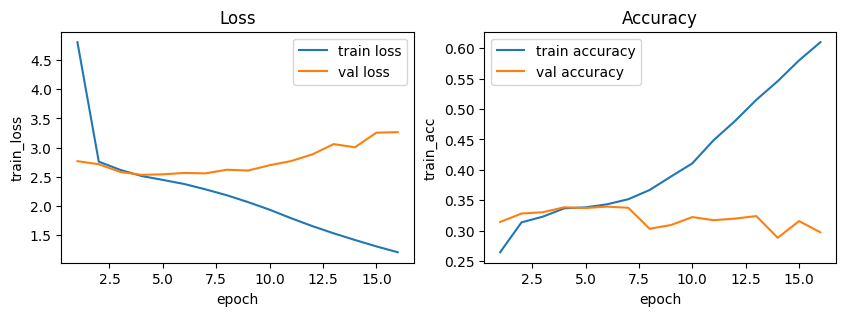
\includegraphics[width=8cm]{img/train_val_loss.png}
\caption{Training and validation loss/accuracy plot for regularized CNN architecture}
\label{fig: train_val}
\end{figure}
% end figure

% start figure
\begin{figure*}[]
\begin{center}

\centering
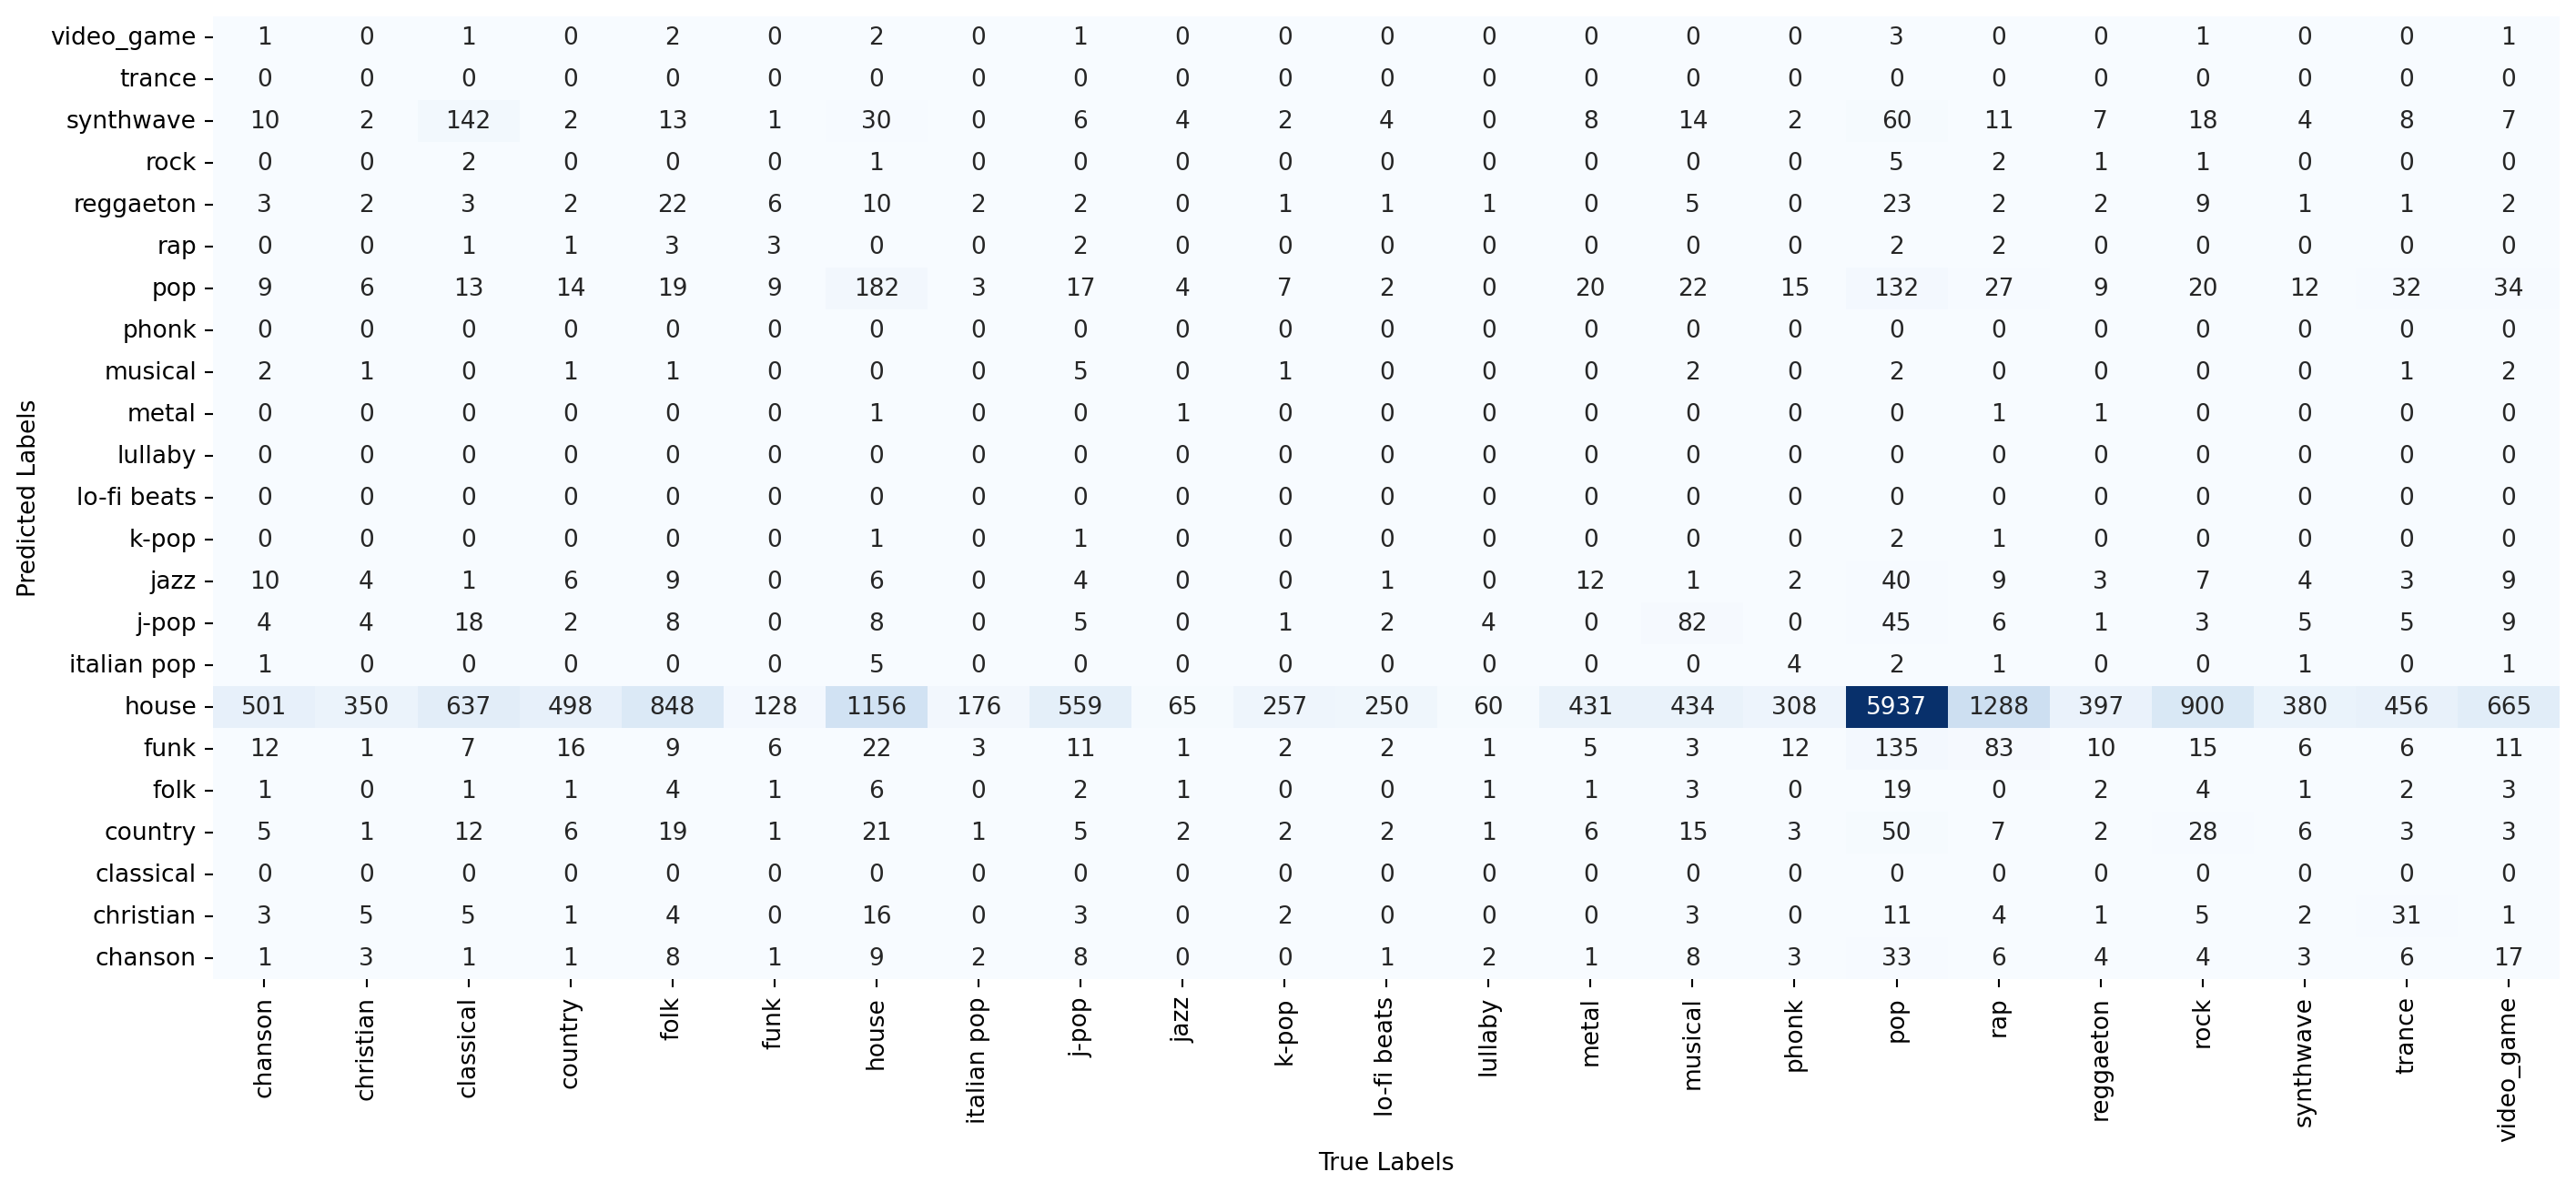
\includegraphics[width=13cm]{img/prediction_test_set.png}
\caption{Heat-map representation for a comparison of predictions and true labels on album cover data-set}
\label{fig: prediction_results}
\end{center}
\end{figure*}
% end figure

Given these premises, we decided to train the regularized version of the CNN for 6 epochs on the entire defined training set and assess its result on the test set. We obtained a final 34.45\% test accuracy and we depict in Figure \ref{fig: prediction_results} a heat-map relating true labels and predicted labels. We notice how, in terms of prediction tendency, the model is completely skewed towards the house music genres, especially in terms of classifying pop music and rap music. This at least allows us to identify the problem of genre classification in this particular image-dataset, emphasizing a negative result and leaving space for further research focusing on facing this issue.


\section{Discussion}

\subsection{Network collection, characterization and preliminary tasks}
In this report, we focused on analyzing a Spotify artists network using network science quantitative tools.

\begin{itemize}
    
\item CM and BA are the two models which fits the AN degree distribution better then the other synthetic graphs tested. We notice how both AN and its synthetic counterparts are in a connected regime, with average degree very close to $ln(N)$.
\item The AN network tends to have a higher average local clustering coefficient when compared with its synthetic counterparts, but all graphs have very low density values. It also shows the highest estimated diameter and average shortest path compared to synthetic models.
\item In terms of community discovery, Louvain proved to be the best method in terms of quantitative internal evaluation measures. The comparison of normalized F-1 scores did not indicate significant similarity with other community detection algorithms used for the analysis. We also observe how the communities found by Louvain relatively capture homogeneous genres when the analysis is made at a coarser-grain level.
\item SimRank proved to be the best unsupervised approach for performing link prediction on the sub-sample of edges extracted from the main dataset. On the other hand, Logistic Regression with the Hadamard operator achieved the best result in a supervised context.

\end{itemize}

\subsection{Artists’ Genres Through the Lens of Album Artwork}
We focused on understanding if any relevant information could be extracted about the artist network relating the communities identified through Louvain algorithm and the albums' artwork: 

\begin{itemize}
    
\item We notice how purest communities in terms of sentiment are mainly characterized by positive images, following the approach discussed in \cite{Vadicamo_2017_ICCV}. Less interpretable an reliable results are available in terms of image classification, and we also underline the weak correlation in terms of purity between image, genre and sentiment.

\item Concept modeling allowed us to unveil a general common tendency among different Louvain genres communities: the fact that most communities' albums can be described either in terms of artistic/visual representation or artists close-ups/full-length photos. 

\item A simple CNN architecture was trained in order to predict the Louvain music genre based on albums artwork: results were unsatisfactory. We speculate that either the labeling is ill-defined or there is no precise and strict correlation between albums' artworks and music genres. Further research would allow us to better understand if these questions have a positive or negative answer

\subsection{Future Work}
Discussing future work in terms of Spotify network analysis, there lies potential in obtaining more insightful information by expanding the network size and extracting additional album images for individual artists. This would contribute to enhancing the dataset available for the genre classification task. Moreover, incorporating textual information alongside images presents an avenue for improvement: considering the most pertinent lyrics from an artist's songs could enhance the genre prediction task within a multimodal framework.

\end{itemize}


% The next two lines define the bibliography style to be used, and the bibliography file.
\bibliographystyle{ACM-Reference-Format}
\bibliography{biblio}

\end{document}
